\documentclass[a4paper,twoside,openright,draft]{memoir}

%% We need to follow NUIG structure and style in the thesis.  They
%% tell us how to do it but they don't really give a template or latex
%% document class to use.  I guess being able to format a document is
%% part.  Follows their documentation retrieved from ``University
%% Guidelines for Research Degree Programmes --- For Research
%% Students, Supervisors and Staff'', July 2016 edition, retrieved on
%% Mon 6 Feb 23:05:05 GMT 2017 from
%% HTTP://www.nuigalway.ie/media/graduatestudies/files/university_guidelines_for_research_degree_programmes.pdf
%%
%% From Section 6 - The PhD Examination Process
%%
%% 6.2.3 Directions on Format, Layout and Presentation
%%
%% The PhD thesis should not normally exceed 80,000 words, inclusive
%% of appendices, footnotes, tables and bibliography.  It is
%% university policy that the practice of engaging professional
%% editorial services to assist in writing the thesis is not
%% permitted.  There must be a title page which shall contain the
%% following information:
%%
%%  a. The full title (and subtitle, if any)
%%  b. The volume number and total number of volumes, if more than one
%%  c. The full name of the candidate, followed, if desired, by any
%%     degree and/or professional qualification(s)
%%  d. The name(s) of the supervisor(s), School(s), component
%%     Discipline(s), Institution
%%  e. The month and year of submission.
%%
%% Format and Layout
%%
%% The 'Table of Contents', which should not be over-detailed, shall
%% immediately follow the title page.  The text must be printed on good
%% quality (110g/m2) A4 size paper.  Line-spacing should be a maximum
%% of one-and-half; text must be left justified with a left-hand
%% margin of 4 cm and may be right justified.  An easily-readable
%% layout and double-sided printing are recommended for the body text.
%% For double sided printing ensure that the right hand margin is also
%% adequate for binding (i.e. a margin of 4 cm).  More compact formats,
%% with smaller font sizes, are usually appropriate for certain
%% sections, such as reference lists, bibliographies and some kinds of
%% appendices.  Pages must be numbered consecutively, with page numbers
%% located centrally at the bottom, and chapter headers at the top, of
%% each page.  Diagrams, graphs, photographs and tables should be
%% properly numbered and located in relation to the text.  The copies
%% of the thesis presented initially for examination must be spiral or
%% gum-bound.
%%
%% This is pretty much repeated in Appendix 1 --- Regulations for
%% Higher Research Degrees, Section 10 Submission of the Thesis.

\chapterstyle{veelo}

\OnehalfSpacing

\makepagestyle{NUIG}
\makeevenfoot{NUIG}{}{\thepage}{} % page numbers in the centre
\makeoddfoot{NUIG}{}{\thepage}{} % page numbers at the centre
\makeevenhead{NUIG}{\leftmark}{}{} % page marks in the edge
\makeoddhead{NUIG}{}{}{\rightmark} % page marks in the edge
\pagestyle{NUIG}

%% Use our NUIG page style, even in pages with a chapter heading.
\aliaspagestyle{chapter}{NUIG}

%% For some reason, the page with the abstract keeps the header with
%% the last page mark (The last "Table of ...").  We don't want to
%% have anything other than the page number on the center as per NUIG
%% requirements.
\copypagestyle{abstract}{empty}
\makeevenfoot{abstract}{}{\thepage}{} % page numbers in the centre
\makeoddfoot{abstract}{}{\thepage}{} % page numbers at the centre

%% NUIG only requires 4cm margin on the spine margin, the rest it's
%% set to whatever makes Andrew happy.
\setlrmarginsandblock{4cm}{3cm}{*}
\setulmarginsandblock{3.5cm}{3.0cm}{*}
\checkandfixthelayout

\usepackage[final,hyperindex,hyperfootnotes,bookmarksnumbered]{hyperref}

\usepackage[T1]{fontenc}
\usepackage[utf8]{inputenc}
\usepackage{textcomp}

\usepackage{palatino}
\usepackage[euler]{textgreek}

\maxtocdepth{subsection}

\usepackage[final]{graphicx}

%% Input files that input others relative to themselves instead of
%% relative to the initial tex file.  Handy for each chapter but an
%% absolute requirement to include the pdf_tex figures from inkscape
%% which call includegraphics with the filename only.
\usepackage{import}

\usepackage{amsmath}

\usepackage[textsize=footnotesize]{todonotes}
  %% new command for box about missing references
  \newcommand{\addref}[1]{\todo[color=red!40,size=\tiny]{Add reference: #1}}

%% Provides multicols environment to create itemize list with multiple
%% columns.
\usepackage{multicol}

\usepackage{enumitem}       % so we can use the unboxed style when item names are too long
\usepackage{longtable}      % because memoir's ctabular does not work well with eqparbox
\usepackage{eqparbox}       % for adjusting size of table column (specially on appendices)
  %% Checks what LaTeX thinks is best for a column and save that value.
  %% It will then use it to calculate what's left of \textwidth, and
  %% use it for the other columns. See http://tex.stackexchange.com/questions/95397
  \newsavebox{\SolutionNameBox}
  \newcolumntype{\SolutionNameCol}{
    >{\begin{lrbox}{\SolutionNameBox}}l<{\end{lrbox}
    \eqmakebox[SolutionNameBox][l]{\unhcopy\SolutionNameBox}}
  }

\usepackage{tikz}

\newsubfloat{figure}        % subfigures with LaTeX

\usepackage{rotating}       % for sideways tables and figures
  \newcommand{\crows}[1]{\multicolumn{2}{c}{#1}}

%% Use agu style (American Geophysical Union) which only uses author
%% forenames and after too many authors, uses et. al.  All this helps
%% saves a lot of paper.
\usepackage[round]{natbib}
\bibliographystyle{agu}

\usepackage{seqsplit}
\usepackage{dnaseq}

\usepackage[binary-units=true]{siunitx}
  \DeclareSIUnit{\gn}{\textit{g$_n$}}   % standard gravity
  \DeclareSIUnit{\bp}{bp}               % base pairs
  \DeclareSIUnit{\cfu}{cfu}             % colony forming unit
  \DeclareSIUnit{\Molar}{\textsc{m}}
  \DeclareSIUnit{\mm}{\si{\milli}\si{\meter}}
  \DeclareSIUnit{\mM}{\si{\milli}\si{\Molar}}
  \DeclareSIUnit{\uM}{\si{\micro}\si{\Molar}}
  \DeclareSIUnit{\X}{\times}
  \newcommand{\dc}[1]{\SI{#1}{\degreeCelsius}}
  \newcommand{\pcent}[1]{\SI{#1}{\percent}}

%% This commands include the caption short description at the start of
%% long description and in bold.
\newcommand{\captionIntro}[2]{\caption[#1]{\textbf{#1.} #2}}
\newcommand{\captionofIntro}[3]{\captionof{#1}[#2]{\textbf{#2.} #3}}

%% Controls the background color of shaded environment (part of memoir
%% document class, similar to the framed package)
\definecolor{shadecolor}{gray}{0.9}

%% Just like we have cite and citep to cite in text and between parentheses,
%% have the same for fref, tref, etc...
\newcommand{\frefp}[1]{(\fref{#1})}
\newcommand{\trefp}[1]{(\tref{#1})}
\newcommand{\Crefp}[1]{(\Cref{#1})}
\newcommand{\Srefp}[1]{(\Sref{#1})}
\newcommand{\Arefp}[1]{(\Aref{#1})}

%% Use for command line name, function names, etc
\newcommand{\command}[1]{\texttt{#1}}

\newcommand{\species}[1]{\textit{#1}}

%% NCBI Style Guide, Chapter 5 "Style Points and Conventions", recommends
%% italic for gene names (except in long list of genes), and roman for
%% protein names.
\newcommand{\gene}[1]{\textit{#1}}
\newcommand{\protein}[1]{#1}

\newcommand{\Kon}{$K_{on}$}
\newcommand{\Koff}{$K_{off}$}
\newcommand{\halflife}[1][]{$t_{1/2}$#1}

\newcommand{\G}[1]{G$_#1$}  % for G0, G1, and G2 phases

\renewcommand{\abstractname}{Summary}

%% make it easy to center any dedication
\newcommand{\dedication}[1]{
{\clearpage\mbox{}\vfill\centering #1 \par\vfill\clearpage}}

\usepackage{makecell}
\usepackage[UKenglish,abbreviations]{foreign}

\input{methods/results/software_versions}

%% Seems like subinputfrom (import package) does not work so well in
%% the preamble, so we still have to specify the full path on the
%% filename.  Relative paths inside the input'ed' files works fine.
\subinputfrom{histone-catalogue/}{histone-catalogue/preamble}

\author{David Miguel Susano Pinto}
\newcommand{\supervisor}{Dr.~Andrew Flaus}
\newcommand{\cosupervisor}{Prof.~Kevin Sullivan}
\date{March 2013} % hopefully
\title{1461 days of rain} % working title for a build without errors
%% TODO possible titles
%%
%% Structure--function relationships in chromatin probed by quantitative dynamics in live cell nuclei.
%% Does not account for the the histone cataloguing part. Plus there wasn't that much
%% study on the structure function relationships as it was mostly methods and things not
%% working great...
%%
%% the main thing behind the thesis is automation (we are not monkeys) and quantitative analysis. Those
%% two words should probably go on the title

\begin{document}
  \frontmatter

  \maketitle

  \dedication{The leprechaun made me do it.}

  \clearpage
  \tableofcontents
  \clearpage
  \listoffigures
  \clearpage
  \listoftables

  \clearpage
  \begin{abstract}  % limit of 300 words

    Chromatin is a dynamic complex that controls access to genetic information by
    undergoing structural reconfigurations. Understanding this dynamics will give
    us a better insight into the biological implications of chromatin organization.

    Quantitative fluorescence microscopy has been used extensively to obtain insights
    into the dynamics of multiple proteins in live cells. Despite the large advances on
    model design, fluorophores and imaging capabilities, limitations are still
    encountered that can lead to misinterpretation of data.

    By using histone proteins with extremely slow exchanging rates we have tested the
    limitations of Fluorescence Recovery After Photobleaching (FRAP) and developed
    approaches to overcome some of them. Importantly, we have shown that movement of
    chromatin does not allow for measurements of histone dynamics on the FRAP time scale.

    By combining FRAP with a FRAP variant technique using photoactivatable proteins, we have
    set up a framework for a new model capable to simultaneously estimate both \Kon{}
    and \Koff{}. For this purpose we have tested the photoconvertible protein mEos2,
    and then constructed a new fluorescent protein combining PA--GFP with mRuby in tandem,
    to avoid the limitations of mEos2.

    Finally, we have undertaken a detailed catalogue of the human histone genes and completed
    their annotations. Based on the ``reproducible research'' concept, we made this
    catalogue not only a self-updatable paper, but also a model for similar projects
    which can be continually improved driven by genome annotations. As proof of concept, we
    are making a catalogue of the current mouse and chicken histone genes by minimal
    adjustment of the code we produced for the human homologues.

    In these studies we have tested the limits of several existing models by designing
    novel reagents, software and approaches in the field of chromatin dynamics.

  \end{abstract}

  \mainmatter

  \chapter{Introduction}
  \subinputfrom{intro/}{intro}

  \chapter{Materials and Methods}
\label{ch:methods}

  \epigraph{As palavras que nunca te direi.}{Translation of ``Message in a bottle''}
  \noindent
  %% "The devil is in the details."

  All chemicals used were purchased from Sigma unless otherwise stated. All
  solutions were prepared according to \Aref{app:solutions} with Milli-Q
  purified water, and autoclaved prior to use when appropriate.

  Restriction enzymes, T4 DNA ligase, other DNA modifying enzymes, and DNA
  ladders were obtained from New England BioLabs. Protein ladders from Invitrogen.

  For use in tissue culture, FCS and DMEM (without phenol red and L-glutamine)
  were obtained from Lonza; DMEM (supplemented with glucose, sodium pyruvate,
  L-glutamine and phenol red), Non-Essential Amino Acid (NEAA) solution, and
  PBS (without Ca$^{2+}$ and Mg$^{2+}$) from Sigma; Penicillin--Streptomycin
  solution and Trypsin-EDTA from Gibco.

  \section{DNA methods}
    \subsection{Bacterial cultures}
      \species{E.~coli} cultures were prepared with either LB broth or agar
      at \dc{37}. For antibiotic selection, ampicillin, kanamycin, and
      chloramphenicol, were used at concentrations of 100, 30,
      and \SI{34}{\mg\per\l} respectively.

    \subsection{Preparation of competent bacteria}
      Competent \species{E.~coli} cells were prepared from a culture of
      Invitrogen's One Shot TOP10 Chemically Competent \species{E.~coli}. LB
      cultures of \SI{1}{\l} were set at \dc{37} until an OD$_{\SI{600}{\nm}}$
      of \numrange{0.4}{0.5}. Further steps were carried at \dc{4} with
      previously chilled equipment and solutions.

      Cultures were centrifuged at \SI{6000}{\gn} for 10 minutes, the
      pellet resuspended in \SI{500}{\ml} of \SI{0.1}{\mM} CaCl$_2$, and
      incubated on ice for 30 minutes. The suspensions were centrifuged
      again at \SI{6000}{\gn} for 10 minutes, and the new pellet resuspended in
      \SI{100}{\ml} of CaCl$_2$ with \pcent{15} glycerol. Aliquots of
      competent cells were prepared and stored at \dc{-80}.

      Transformation efficiencies were measured after preparation of each
      batch and discarded if less than \SI{1d6}{\cfu\per\mg} of plasmid was
      obtained. Absence of antibiotic-resistant contaminations was assessed
      by streaking the cells on selective plates.

    \subsection{Transformation of competent cells}
      Competent cells were thawed on ice and split into aliquots of
      \SI{50}{\ul} to pre-chilled \SI{2}{\ml} tubes where \SI{1}{\ul} DNA
      was added. Cells were incubated on ice for 30 minutes, followed by a
      60 seconds heat-shock at \dc{42}, and 5 more minutes on ice.
      \SI{300}{\ul} of non-selective LB was added to each tube and the
      cultures incubated at \dc{37} with vigorous shaking for 45 minutes.
      Samples from the cultures were plated onto the appropriate
      antibiotic containing plates, and incubated overnight at \dc{37}.

      For concentrations of plasmid DNA higher than \SI{500}{\ng\per\ug}, only
      \SI{0.3}{\ul} of DNA was used, and both the initial and final incubation
      steps were shorten to 10 minutes.

    \subsection{Plasmid DNA preparation}
      Plasmid DNA was prepared with kits QIAprep Spin Miniprep,
      QIAGEN Plasmid \textit{Plus} Midi, QIAquick Gel Extraction, and QIAquick
      PCR purification from QIAGEN following the manufacturer's instructions.
      Once prepared, DNA was stored at \dc{-20}. DNA concentrations were measured
      with a spectrophotometer (NanoDrop 2000c spectrophotometer from
      Thermo Scientific).

    \subsection{Ethanol precipitation}
      \label{sec:ethanol-precipitation}
      The DNA solution was mixed with \num{2.5} volumes of \pcent{100} ethanol
      and \num{1/10} volumes of Sodium Acetate (\SI{3}{\Molar}, pH=\num{5.2}),
      and incubated at \dc{4} for 15 minutes. When DNA concentrations was below
      \SI{50}{\ng\per\ug}, incubation was performed overnight.
      Solution was centrifuged at
      \SI{18000}{\gn} for 30 minutes at \dc{4}, the supernatant discarded, and
      the pellet left to dry until all traces of solvent evaporated. DNA pellet
      was resuspended in the desired solvent: H$_2$O when used for transfection,
      EB~buffer from QIAGEN otherwise.
      low DNA plasmid concentrations)

    \subsection{Agarose gels electrophoresis}
      Agarose gels with concentrations ranging from \SIrange{0.6}{2.0}{\percent}
      were prepared with TAE buffer, and supplemented with ethidium bromide.
      DNA samples were loaded into the gel with DNA loading buffer and a
      choice of loading dyes between bromophenol blue, cresol red, orange G, or
      xylene cyanol, to avoid shadowing of the DNA bands. Electrophoresis was
      performed in electrophoresis chambers with \SI{1}{\X}~TAE buffer at
      \SIrange{80}{120}{\volt} until the required separation was achieved.
      Gels were visualized at an UV transilluminator ChemiImager 5500 from
      Alpha Innotech.

    \subsection{DNA sequencing and oligonucleotide preparation}
      DNA sequencing was performed by LGC Genomics after cloning for sequence
      confirmation and avoiding unexpected mutations.

      Oligonucleotides were ordered from Eurofins MWG operon in lyophilized
      format, dissolved in H$_2$O to a \SI{100}{\micro\Molar} concentration,
      and stored at \dc{-20}. A list of all designed oligonucleotides is
      produced at \Aref{app:primers}.

    \subsection{Polimerase Chain Reaction}
      Different types of PCR experiments were performed for different purposes
      with different DNA polymerases (\tref{tab:pcr-settings}). Taq with ThermoPol
      buffer was obtained from New England Biolabs. KOD Hot Start with Mg$^{2+}$
      free buffer was obtained from Novagen. PCRs were performed on a thermocycler
      Mastercycler epgradient from Eppendorf.

      Use of different DNA polymerases was based on their cost-benefit for
      each application. For example, screening clones requires a large number
      of reactions in simultaneous and the introduction of small mutations
      is of no consequence. For this two reasons, the much cheaper Taq DNA
      polymerase was used for screening despite its low fidelity and
      amplification rates. However, in PCR mutagenesis the whole plasmid
      is synthesized anew and we have no reasonable method to verify its whole
      sequence. As a result, KOD DNA polymerase was used for PCR mutagenesis.

      \begin{sidewaystable}
        \centering
        \captionIntro{PCR mixtures and conditions used.}
          {
            Since each reaction was unique, with different pair of primers
            and template DNA, the optimal salt concentrations, temperature
            of the annealing step, and time of extension step actually used were
            sometimes different. Listed values correspond to the standard
            usage and initial attempts.
          }
        \label{tab:pcr-settings}

        \newcolumntype{W}{r<{\si{\second}}}
        \newcolumntype{T}{l<{\si{\degreeCelsius}}}

        \begin{tabular}{l W@{ at }T W@{ at }T W@{ at }T W@{ at }T W@{ at }T}
          \toprule
          \null                        & \multicolumn{4}{c}{cloning} & \crows{colony} & \crows{mutagenesis} & \crows{screening} \\
                                                \cmidrule(r){2-5}
          \null                        & \crows{genomic} & \crows{plasmid} \\
          \midrule
          Template (\si{\ng})          & \crows{1000}      & \crows{50}        & \crows{n/a}       & \crows{750}       & \crows{50}        \\
          DMSO (\si{\ul})              & \crows{---}       & \crows{---}       & \crows{1}         & \crows{---}       & \crows{1}         \\
          Buffer (\si{\X})             & \crows{1}         & \crows{1}         & \crows{1}         & \crows{1}         & \crows{1}         \\
          MgSO$_4$ (\si{\nmol})        & \crows{1.5}       & \crows{1.5}       & \crows{---}       & \crows{1.5}       & \crows{---}       \\
          dNTPs (\si{\mM} each)        & \crows{0.2}       & \crows{0.2}       & \crows{0.2}       & \crows{0.2}       & \crows{0.2}       \\
          Primer (forward) (\si{\uM})  & \crows{2}         & \crows{2}         & \crows{2}         & \crows{0.4}       & \crows{2}         \\
          Primer (reverse) (\si{\uM})  & \crows{2}         & \crows{2}         & \crows{2}         & \crows{0.4}       & \crows{2}         \\
          DNA polymerase (\si{U})      & \crows{0.5 (KOD)} & \crows{0.5 (KOD)} & \crows{2.5 (Taq)} & \crows{0.5 (KOD)} & \crows{2.5 (Taq)} \\
          \addlinespace
          Total volume (\si{\ul})      & \crows{25}        & \crows{25}        & \crows{25}        & \crows{25}        & \crows{25}        \\
          \addlinespace
          \midrule
          \addlinespace
          Initialization                & 120 & 94    & 120 & 94    & 180 & 94    & 120 & 94    & 120 & 94 \\
          Denaturation                  &  30 & 94    &  30 & 94    &  15 & 94    &  30 & 94    &  15 & 94 \\
          Annealing                     &  20 & 58    &  20 & 58    &  15 & 58    &  20 & 58    &  15 & 62 \\
          Extension (per \si{\kilo\bp}) &  30 & 68    &  20 & 72    &  60 & 72    &  30 & 68    &  60 & 72 \\
          Final extension               & 300 & 62    & 300 & 72    & 300 & 72    & 300 & 94    & 300 & 72 \\
          Final hold       & \crows{\dc{4}}      & \crows{\dc{4}}      & \crows{\dc{4}}      & \crows{\dc{4}}      & \crows{\dc{4}} \\
          Number of cycles & \crows{\SI{30}{\X}} & \crows{\SI{30}{\X}} & \crows{\SI{30}{\X}} & \crows{\SI{15}{\X}} & \crows{\SI{20}{\X}} \\
          \bottomrule
        \end{tabular}
      \end{sidewaystable}

      \subsubsection{Colony PCR}
        When screening multiple clones after transformation and a set of
        appropriate primers was available, PCRs were set directly from
        the bacteria colonies by adding them directly to the reaction mixture
        (\tref{tab:pcr-settings}). Bacteria from individual colonies were
        used to simultaneously perform a PCR and start a small culture.
        Plasmid purification was performed on cultures whose sample was
        positive by PCR.

      \subsubsection{Gene cloning}
        PCRs were used to clone and subclone genes from genomic DNA and
        plasmids, into different vectors. The most commonly used vectors
        were pEF--BOS, pEGFP-C1, pEGFP-N1, pET3, and pET15 but a complete
        list is displayed on \Aref{app:plasmids}. Primers were usually
        extended to engineer restriction sites and create DNA linkers but
        were even longer on the 5' end to account for the minimum
        required \si{\bp} around the restriction sites \citep{neb_catalogue_2011}.

      \subsubsection{Mutagenesis}
        PCR mutagenesis
        \footnote{
          In PCR mutagenesis, since the newly synthesized strands will
          be linear and cannot be used as template, the amplification
          is linear rather than exponential. Because of this, the name
          PCR mutagenesis is misleading. There is \emph{no} actual chain reaction.
        }
        was used to insert or correct mutations in plasmids. When choice
        was possible, the selected codon used for mutation was the one
        with highest frequency in the expressing organism, following the
        codon usage database \citep{codon_usage}. After amplification,
        \SI{1.5}{\ul} of restriction enzyme DpnI
        \footnote{
          Because DpnI activity is blocked by DNA methylation, it will
          only digest the template DNA which was synthesized in bacteria,
          leaving the newly \textit{in vitro} synthesized DNA intact.
        }
        was added directly to the PCR mixture, and incubated overnight at
        \dc{37}. \SI{1}{\ul} was used for transformation and individual
        clones screened by sequencing.

      \subsubsection{Screening plasmid}
        PCRs were frequently used to screen plasmids for DNA sequences
        in the absence of opportune restriction sites or even plasmid maps.

  \section{Protein methods}
    \subsection{Phenol:chloroform extraction}
      \label{sec:phenol-extraction}
      To extract proteins, an equal volume of phenol:chloroform was
      added and the mixture centrifuged at \SI{6000}{\gn} for 15 minutes.
      The top aqueous phase (chloroform) was pipetted to a new tube and
      the process repeated a total of 3 times.

    \subsection{Western blotting}
      \subsubsection{Protein concentration determination}
        Concentration of protein was measured with Bradford reagent.
        \SI{2}{\ul} of the sample after sonication (\Sref{sec:cell-extract})
        was mixed with \SI{48}{\ul} of H$_2$O and \SI{50}{\ul} of NaOH and
        incubated at \dc{65} for 8 minutes before adding \SI{900}{\ul} of
        Bradford reagent from Pierce. The mixture was transferred to plastic
        cuvettes and the absorbance at \SI{595}{\nm} measured in a Shimadzu
        spectrophotometer. The values obtained were interpolated from a
        standard curve prepared using known concentrations of BSA.

      \subsubsection{SDS--PAGE}
        Resolving and stacking SDS--PAGE gels of \SIrange{15}{5}{\percent}
        respectively, both with a cross-linking ratio of \num{37.5}:1 as
        described in \citet{harlow_electrophoresis_1988}. The
        resolving gel was poured directly after addition
        of TEMED and it was covered with a layer of isopropanol during polymerisation
        to ensure a sharp interface between the resolving and stacking layers.
        Protein samples and markers were boiled at \dc{99} for 3 minutes and each
        was loaded twice, with volumes for \SI{3.3}{\ug} and \SI{16.5}{\ug} of
        protein. Gels ran at \SI{180}{\volt} for 1 hour in \SI{1}{\X} TG buffer.

      \subsubsection{Protein transfer}
        Protein transfer occurred through the wet transfer system. The
        SDS-PAGE gel was placed onto pre-cut nitrocellulose transfer membrane
        previously soaked in transfer buffer. It was then set between a pair
        of extra thick blotting paper and cushions before being placed inside
        a transfer apparatus. The transfer ran at \dc{4} for 60 minutes.

      \subsubsection{Probing of blot with antibody}
        Blocking of the membrane was performed with \SI{10}{\percent}
        non-fat dry milk in \SI{1}{\X} TBST
        at room temperature for 30 minutes. Blocking was followed by
        primary antibody incubation which occurred in \SI{5}{\percent} non-fat
        dry milk in \SI{1}{\X} TBST overnight at \dc{4}. Concentrations of
        antibody used were 1:500 and 1:20000 for anti-GFP (catalogue
        number 11~814~460~001 from Roche) and anti-H3 (code ab1791 from
        abcam). The membrane was then washed with \SI{1}{\X} TBST for
        15 minutes 3 times before the secondary antibody incubation which
        occurred in \SI{5}{\percent} non-fat dry milk in \SI{1}{\X} TBST for
        1 hour. The membrane was washed once more in the same
        conditions as before for the detection. All blocking, antibody
        incubation and washing steps occurred on a rocker.

        Detection was performed using the SuperSignal West Pico Chemiluminescent
        Substrate from Pierce, adding 1:1 of the solutions and allowing it to incubate
        with the membrane for 5 minutes. The membrane was exposed to x-ray films for
        10, 60, 5, 180 and 1800 seconds which were then developed.


  \section{Cell methods}
    \subsection{Cell culture}
      HeLa and HEp-2 cells were supplied by Agnieszka Kaczmarczyk from the
      National University of Ireland, Galway, Department of Biochemistry,
      and Volker D\"oring from the Leibniz Institute for Age Research -- Fritz Lipmann Institute.
      Primary horse fibrolasts were a gift from Prof.~Elena Giulotto from the
      University of Pavia, Department of Genetics and Microbiology.

      All cell lines were maintained at \dc{37} and \pcent{5} CO$_2$ in \SI{10}{\cm}
      diameter plates with \SI{10}{\ml} of their respective growth medium (see \Aref{app:solutions}).
      Dulbecco's Phosphate Buffered
      Saline (DPBS) and trypsin--EDTA solutions were used, respectively, to wash
      and split the cells 1:10 once they reached a confluence of \SIrange{80}{90}{\percent}.

    \subsection{Cell stock storage}
      For long-term storage of HeLa cell lines, they were grown until
      they reached a confluence of \SIrange{80}{90}{\percent} and then
      trypsinized as usual. A volume of Freezing Media was added, equal
      to the volume of trypsin--EDTA, and \SI{2}{\ml} aliquots of
      cells transferred to cryotubes. Tubes were immediately wrapped in
      cotton and placed at \dc{-80}.

    \subsection{Whole cell extract}
      \label{sec:cell-extract}
      To obtain whole cell extracts, HeLa cells were trypsinized as usual. Growth
      medium added and the suspension was centrifuged at \SI{900}{\gn}
      for 10 minutes. Further steps were carried at \dc{4} and with previously
      chilled reagents. The supernatant was discarded and the pellet
      resuspended in \SI{500}{\ul} of chilled PBS before being
      sonicated 3 times at \pcent{40} amplitude for 10 seconds. Avoiding the
      foam formed at the top, \SI{300}{\ul} of suspension were transferred
      from the bottom of the tube to a new eppendorf and mixed with an equal
      volume of Laemmli buffer before being stored at \dc{-80}.
      \SI{2}{\ul} from the suspension was also transferred to a new tube
      for determination of protein concentration.

    \subsection{Genomic DNA extraction}
      To extract genomic DNA of HeLa cells, they were trypsinized as usual and
      growth medium was added in the end before counting with an hemocytometer.
      Cells were centrifuged at \SI{1500}{\gn} for 10 minutes at \dc{4}, the
      supernatant discarded and the pellet resuspended in TE buffer to achieve
      a desired concentration of \SI{4e7}{cells\per\ml}. 9 volumes of
      Genomic lysis buffer was added and the mixture incubated at \dc{37} for
      90 minutes. Proteinase K was added to a final concentration of
      \SI{100}{\ug\per\ml} and the mixture incubated at 50 °C for 3 hours and
      swirled every 20 minutes. DNA was then extracted by
      phenol:chloroform (\Sref{sec:phenol-extraction}) and purified by ethanol
      precipitation (\Sref{sec:ethanol-precipitation}).

    \subsection{Viable cells count}
      \label{sec:methods:trypan-blue}
      Trypan blue was used to assess the number of viable cells.
      After trypsinization as usual, cells were diluted in growth medium,
      to a final concentration of \SI{2e5}{cells\per\ml}.
      To \SI{0.5}{\ml} of the cell suspension, was added \SI{0.1}{\ml}
      of \pcent{0.4} Trypan Blue Stain and the mixture left for 5 minutes
      at room temperature before counting
      the cells in an hemocytometer making a distinction between
      stained (non-viable) and non-stained (viable) cells.

    \subsection{Kill curve}
      \label{sec:methods:kill-curve}
      Cells were trypsinized as usual and plated at \pcent{25} confluence on
      a 24-well plate. After 24 hours, medium was replaced using different
      concentrations of the antibiotic per well, 3 replicas for each.
      After 3 days, medium was
      renovated with the same antibiotic concentrations. After 4 days, total of
      one week after addition of antibiotics, cells were trypsinized and a count
      of viable cells was performed with Trypan Blue (\Sref{sec:methods:trypan-blue}).

      The highest concentration tested with no viable cells in all replicas after
      7 days, was used for selection of transfected cells when establishing
      stable cell lines.

    \subsection{Transfection by lipofection}
      \label{methods:lipofection}
      Cells were transfected using Lipofectamine~2000, a cationic lipid
      reagent, from Invitrogen. Cells were trypsinized as usual on the
      day before transfection and replated on 6 well plates (surface area
      of \SI{9.5}{\square\cm\per well}) with \SI{2.5}{\ml} of growth
      medium so they would be \SI{90}{\percent} confluent on the following
      day. For each well, two tubes with \SI{250}{\ul} of transfection
      medium were prepared, one with \SI{7.5}{\ul} of Lipofectamine~2000
      and another with \SI{3750}{\ng} of DNA from a stock with concentration
      of \SI{500}{\ng\per\ul} and prepared by ethanol precipitation
      (\Sref{sec:ethanol-precipitation}).
      Both tubes were incubated at room temperature for 5 minutes,
      mixed together, and incubated again at room temperature for 20 minutes. Cells
      were washed with DPBS during this time and growth medium switched to \SI{2}{\ml}
      of transfection medium. The mixture was then added to the cells medium who
      were incubated at \dc{37} for 6 hours after which time it was switched back to
      \SI{0.5}{\ml} of growth medium.

    \subsection{Transfection by electroporation}
      Cells were transfected by electroporation using an Amaxa nucleofector
      device with Ingenio Electroporation solution and cuvettes from Mirus Bio.
      Cells were grown to confluence and trypsinized as usual. Growth medium was
      added to a total volume of \SI{8}{\ml}, and \SI{1}{\ml} aliquots (for
      approximately \SI{10e6}{cells}) were centrifuged at \SI{160}{\gn} for 5~minutes.
      The supernatant was discarded and a volume of \SI{2}{\ul} of plasmid at
      a concentration of \SI{500}{\ng\per\ul} was added to the top of the pellet.
      The cell pellet was ressuspended in \SI{100}{\ul} of Mirus Bio Ingenio
      Electroporation solution and transferred to \SI{0.2}{\cm} cuvettes for
      electroporation in an Amaxa nucleofector. According to the manufacturers
      instructions, the preset programs I-013 and O-17 were used to transfect
      HeLa and HEp-2 cells respectively.


    \subsection{Fixation and staining}
      For microscopy visualization, cells grown directly on top of HCl washed coverslips since
      HeLa cells have difficulty attaching to glass. At least 24 hours passed
      between the plating and fixation. Growth medium was removed and the cells
      washed with PBS once before incubation with \SI{4}{\percent} formaldehyde in PBS
      for 4 minutes. The solution was removed and the cells washed with H$_2$O 2 more
      times, after which coverslips were removed from the wells and left to air dry.
      For each coverslip, \SI{2}{\ul} of SlowFade Light Antifade kit from Molecular Probes
      was used for mounting the coverslip on a microscope slide. DAPI was added
      to the mounting media when needed. Coverslips were then sealed with a 1:1
      mixture of clear nail polish and acetone and stored on a dark box at \dc{4}.

    \subsection{Flow citometry}

      Cells were trypsinized as usual and after addition of medium, centrifuged
      at \SI{160}{\gn} for 5~minutes. The supernatant was discarded and the
      pellet washed with PBS. The sample was centrifuged one more time at
      \SI{160}{\gn} for 5~minutes. The supernatant was discarded and the
      pellet resuspended in FACS buffer.

      Both sample analysis and cell sorting were performed with live cells, the
      first with a BD FACSCanto~II, and the later with a BD FACSAria~II.

  \section{Software used}
    \label{sec:methods:software}
    The European Molecular Biology Open Software Suite (EMBOSS) version 6.4.0
    was used for analysis of codon usage, RNA folding, and reading of
    chromatogram files.

    The BioPerl and Bio-EUtilities Perl distributions,
    versions \BioPerlVersion{} and \BioEUtilitiesVersion{} respectively,
    were extensively used for analysis and manipulation of biological
    sequences, and automate searches on the Entrez databases.

    Image analysis was performed using GNU Octave version \OctaveVersion{},
    and the Octave Forge image, optim, statistics, bioformats, and signal
    packages, versions \OctaveImageVersion{}, \OctaveOptimVersion{},
    \OctaveStatisticsVersion{}, \OctaveBioformatsVersion{}, and
    \OctaveSignalVersion{} respectively.

    ImageJ, as distributed by the Fiji project, was routinely used
    for microscope image visualization.

  \chapter{Software Tools for Image and Sequence Analysis}

\todo[inline]{Add one page general background to broad needs and
  motivations of software.  Two sections on: Why software development
  is essential for cell biology (1 page), and Why FOSS is important for
  researchers (half page)}

\section{GNU Octave}

The GNU Octave programming language was heavily used for the analysis
of microscope images throughout this work.  Several features of the
language such as its handling of multi-dimensional arrays, interactive
top level, and extensive image processing functions, as well as
its supportive community make it an attractive choice
for quantitative microscopy.

Biological microscope images have a varying number of dimensions.
In addition to the 2 dimensional plane of a standard image, microscope
outputs typically include any combination of: $z$ dimension along
the optical axis for a volume image; time dimension for time-lapse
experiments; and wavelength for multi-channel experiments.  Recent microscopy
techniques generate images with an even higher number of dimensions
such as angle, phase, and lifetime.  This varying dimensionality adds
complexity and makes it challenging to write generalized subroutines for
microscope image analysis.

%% All values are multi-dimensional arrays does not include objects
%% wrapped from other languages such as java objects (and I guess it
%% will be the same for python when the pytave project is finished).
GNU Octave is an array programming language, high level programming
languages where operations are generalised to multidimensional arrays,
primarily intended for numerical computations \citep{octave}.
In Octave, all values are multidimensional arrays which provides
an abstraction layer that is useful when writing code for an arbitrary
number of dimensions as is the case for microscope image processing.

%% Doesn't seem to be any scientific study about REPL as an advantage
%% for prototyping.  Similarly, none about being better for
%% exploratory data analysis but I can't imagine anyone disagreeing
%% with it.
Octave also has a Read--Eval--Print Loop (REPL), or interactive top
level, like IPython and Unix shells, which reduces the
feedback time and provides an efficient
environment for exploratory data analysis.

%% No citation for this, only the anecdotal evidence of being the
%% project leader of octave Forge for 6 years.
The project has a large and active community
mainly composed of
scientists and engineers as a large support group of
specialists in numerical computations.
The separate Octave Forge project hosts a vast number of
packages that extend Octave into specific applications such as control
systems \citep{octave-control}, time-frequency analysis
\citep{octave-ltfat}, or level sets \citep{octave-level-set}.
It provides a collaborative environment for development of Octave
packages and another nexus of the Octave community.

Both GNU Octave and Octave Forge packages are free software which allows
the study, modification, and distribution of modified source.
We made extensive
use of this feature and have contributed to improving Octave and its
packages for the needs of quantitative microscopy.

Finally, Octave comes with basic support for image processing and the
Octave Forge image package extends it with a number of functions for
image processing such as geometric transformations, mathematical
morphology, image registration, and noise reduction.

%% These were actually lsm files but those are actually TIFFs.
While Octave is well suited to image
processing, we also identified several problems always related with
the large image size or number of dimensions.  Our microscopy images
were several megabytes in size.  For example, the single cell
FRAP experiments for histone dynamics generating TIFF files of 449
These images had a field of view of 300
by 300 pixels and 2500 time frames
on acquisition by an 8-bit camera.
Such files sizes are typical in the field of microscopy.

\subsection{Reading and Writing of Image Files}

%% Number of 88 major image formats taken from GraphicsMagick
%% documentation on February 2017.
Octave uses the GraphicsMagick C++ library for the reading and writing
of image files which provides a common interface
to a varied collection of
image format specific libraries covering almost
90 major image formats.  In Octave, this functionality is
provided via the functions \command{imfinfo}, \command{imread}, and
\command{imwrite}.

%% The importance of reading all planes in a single call to imread is
%% of performance for TIFF.  This is because of the structure of TIFFs
%% where reading plane N means parsing all the IFDs before that.
These three functions were rewritten with the aim of achieving
reduced memory usage, increased performance, improved
interface for multidimensional images, and new image types.
New options were added to read and write a series of image planes
in a single function call, to read specific regions of interest in
individual planes, to read and write images
with floating point precision, and to append additional planes to existing image
files.

As part of this rewrite, new features were introduced such as
support for the CMYK colour model, EXIF
and GPS metadata, reading and writing of animations in GIF images, and
control over the image compression type,
while existing features were improved such as
support for transparency and
indexed images.

%% We can't use the term image IO functions because then we would have
%% to explain what IO is.  For the same reason, we can't say ``hooks''.
To support this development, we created a system that allows changing
how the \command{imread}, \command{imwrite}, and \command{imfinfo}
functions behave for each file format.
This enables Octave extensions to add support for new image file
formats or to improve access to the existing formats
without addition of new format specific functions.
For example, it is now possible for packages to enable reading of
microscope specific metadata from \command{imfinfo}.
This system is available via the function \command{imformats}.

Changes extended to other functions of Octave related to images
including  functions involved in conversion between color
models, grayscale images, and indexed images to support integer and
floating point data types, and multiple dimensions
\trefp{tab:software:octave-core-functions}.

All changes were released with Octave version 3.8.0.

\begin{table}
  %% This table includes the major things we contributed to Octave
  %% core.  It doesn't mention a version since it's work I contributed
  %% between Octave 3.6 and 4.2.  Some of the changes even span
  %% multiple versions.
  %% It does not include minor bug fixes or trivial bug fixes.  Also
  %% does not include major changes we did to the internals which only
  %% reduced code duplication.
  \captionIntro{New or improved functions in GNU Octave}{}
  \label{tab:software:octave-core-functions}
  \begin{multicols}{3}
    \begin{itemize}[label={}]
      \foreach \function in {
        bitcmp,
        bzip2,
        cubehelix,
        fliplr,
        flipud,
        flip,
        frame2im,
        gallery,
        gray2ind,
        gzip,
        hsv2rgb,
        im2double,
        im2frame,
        imfinfo,
        imformats,
        imread,
        imwrite,
        ind2gray,
        ind2rgb,
        inputParser,
        ntsc2rgb,
        pkg,
        psi,
        rectint,
        rgb2hsv,
        rgb2ind,
        rgb2ntsc,
        rot90,
        validateattributes}
      { \item \command{\function} }
    \end{itemize}
  \end{multicols}
\end{table}

\subsection{Bio-Formats and Octave Java interface}

%% We kind of managed to read the pixel data.  This also required
%% knowing that LSM interleaves the actual pixel data with thumbnails
%% which need to be skipped.
While GraphicsMagick provides support to read many image formats, its
support for scientific microscope image formats is limited.
For example, Zeiss confocal microscopes saves
images in the LSM file format which is a proprietary extension of TIFF.
Although GraphicsMagick reads LSM pixel data,
the file metadata such as pixel size, time interval, or region of
bleaching event cannot be retrieved.

Bio-Formats is a free software library for reading and writing image
data with a strong focus on microscopy image file formats
\citep{bioformats}.  It is written in the Java programming language and
used by other programs in the field of microscope image analysis such
as CellProfiler \citep{cellprofiler}, ImageJ \citep{imagej2}, and OMERO
\citep{omero}.

%% Before version 3.8.0, there was a separate Octave Forge package
%% that added the java interface.  Actually, Octave version 3.8.0
%% pretty much only merged the java package into it.
Octave has a native interface to the Java programming language
that should enable easy integration with
Bio-Formats, and Bio-Formats has a Matlab toolbox that should be
compatible with Octave.
We identified a series of problems in the Octave interface to Java that
could be solved either by improving Octave or Bio-Formats.

%% Writing this paragraph without mentioning the words data type,
%% primitive, wrapper, and objects is though.  And on top of that,
%% writing it without sounding dumb is just impossible.
In Octave, we rewrote the handling of values returned from Java.
Of special importance for BioFormats was the automatic conversion of
Java arrays which are used to return pixel data.
Support for conversion of multidimensional Java arrays was not implemented
since we did not require it and it remains available for a future project.

In Bio-Formats, we modified their Matlab toolbox so that it is
both Octave and Matlab compatible.
This change simplifies the packaging of
Bio-Formats for Matlab and Octave making them
effectively the same code.
Finally, we automated the creation of Octave packages in Bio-Formats
so that they be made part as part of Bio-Formats releases.

All changes were released with Octave since version 4.0.0 and
Bio-Formats since version 5.1.2

\section{Octave Forge image package}

The Octave programming language is primarily intended for numerical
computations and provides a syntax and set of functions particularly
convenient for solving linear algebra and differential equations.  It
also includes a collection of functions for the handling of image data
but those are focused on the reading and writing of image files,
conversion between colour models, and graphical display.

The Octave Forge image package supplements Octave with a wide range of
image analysis specialised functions.  While Octave syntax is
identical for any number of dimensions and data type, we found that
many of the image package functions were either limited to two
dimensional images or inefficient for the large images we obtained in
microscopy.  We began a project with the purpose of eliminating any
limitation on number of dimensions in the image package
\trefp{tab:software:octave-image-functions} which has seen multiple
releases, starting in version 2.0.0 and continuing in the current
version 2.6.1.
%% Other issues are when functions just treated higher number of
%% dimensions as a long 2D image and introduced artifacts on image
%% borders.  Or they looped over each pixel making it terribly slow
%% even on 2d images.
%%
%% The first time the project to support ND images was made official
%% was for the summer of 2013 (my GSOC) but even on that proposal I
%% mentioned work already made.

\begin{table}
  \captionIntro{New or improved functions in the Octave Forge image
    package}{}
  \label{tab:software:octave-image-functions}
  \begin{multicols}{3}
    \begin{itemize}[label={}]
      \foreach \function in {
        bestblk,
        bwareafilt,
        bwareaopen,
        bwconncomp,
        bwdist,
        bwlabel,
        bwlabeln,
        bwmorph,
        bwperim,
        bwpropfilt,
        checkerboard,
        col2im,
        colfilt,
        conndef,
        edgetaper,
        fftconv2,
        fftconvn,
        grayslice,
        graythresh,
        im2col,
        imabsdiff,
        imadjust,
        imattributes,
        imbothat,
        imclearborder,
        imclose,
        imcomplement,
        imcrop,
        imdilate,
        imerode,
        imfill,
        imgetfile,
        imhist,
        imlincomb,
        immse,
        imopen,
        impixel,
        impyramid,
        imquantize,
        imreconstruct,
        imregionalmax,
        imregionalmin,
        imresize,
        imrotate,
        imtophat,
        intlut,
        iptcheckconn,
        label2rgb,
        labelmatrix,
        mat2gray,
        mmgradm,
        montage,
        nlfilter,
        normxcorr2,
        ordfiltn,
        otf2psf,
        padarray,
        psf2otf,
        psnr,
        regionprops,
        rgb2ycbcr,
        strel,
        stretchlim,
        subimage,
        tiff\_tag\_read,
        watershed,
        wavelength2rgb,
        ycbcr2rgb}
      { \item \command{\function} }
  \end{itemize}
  \end{multicols}
\end{table}

\subsection{Image Thresholding Algorithms}

Image thresholding is a method for image segmentation where the image
pixels are separated into classes based on their intensity values.
The simplest of the thresholding methods uses a single fixed value and
separates an image into background and foreground which are then
represented in a binary, or black and white, image.  This is
particularly useful in images of fluorescence microscopy where objects
of interested show bright with high intensity values against a dark
background with low intensity values.

Multiple threshold algorithms exist to automate the choice of a
threshold value, the most common of which being based on the analysis
of an image histogram \citep{analysis-hist-threshold}.  Otsu's method
\citep{otsu-threshold} is among the most widespread of this methods
and is available in the function \command{graythresh} of the image
package.  We rewrote this function to handle histograms of arbitrary
length, vectorised for performance, and additional computation of a
``goodness'' of the threshold value.  In addition, we ported to Octave
the HistThresh toolbox, an unpublished collection of histogram
threshold algorithms by Antti Niemistö, making them available as an
option for \command{graythresh}.  Finally, the rewrite added the
option of using an histogram as input instead of an image, enabling
the possibility of histogram processing as a preceding step.

%% We have no reference for Antti Niemistö work.  It was never
%% published and only available on his University webpage at
%% http://www.cs.tut.fi/~ant/histthresh/ which is no longer available.
%% He has several other publications but none about this topic.
%% Here's one: A. Niemistö, V. Dunmire, O. Yli-Harja, W. Zhang, and
%% I. Shmulevich, "Robust quantification of in vitro angiogenesis
%% through image analysis," IEEE Transactions on Medical Imaging,
%% vol. 24, no. 4, pp. 549-553, April 2005.
%%
%% The only copies of his work that I know of are on my github account
%% (which I have since modified), and on https://archive.org/web

All this changes have been released with the Octave Forge image
package version 2.0.0.

\subsection{Mathematical Morphology}

%% This is not the complete story.  When we started, imdilate and
%% imerode had some support for ND images.  I can't quite remember
%% what was missing but I do remember making a table at the end with
%% performance comparison, and some comparisons couldn't be made
%% because they were missing before.  Looking at the source for 1.0.15
%% (before I started this), I can see that imerode and imdilate called
%% ordfiltn for grayscale images which was bound to be quite slow, and
%% filter2 for binary images which would limit to 2d images.
Mathematical morphology is the theory for the analysis of spatial
structures which provides a powerful image analysis technique based on
the shape and form of objects.  This is achieved by probing an image
with a known shape, named Structuring Element (SE), and filtering the
image based on whether the SE fits, or does not fit, on each location
within the image.

The fundamental morphological operations are named dilation and
erosion which are available in the image package through the
\command{imdilate} and \command{imerode} functions.  More complex
morphological operations are built on top of this two operations.  For
example, morphological top-hat transform corresponds is the difference
between an image and its morphological opening which in turn
corresponds to an erosion followed by a dilation.

Being the two fundamental operations, they are the ideal targets of
improvements for mathematical morphology since any performance
improvement and support for new image types will be propagated to
other morphology functions.

%% The original imdilate and imerode used __spatial_filtering__ with
%% the ordefiltn option.  We first optimised this by using convn which
%% made it a lot faster but only for binary images.  We then modified
%% __spatial_filtering__ so that it was faster in grayscale images
%% too.  We ended up writing a specialised function for dilation and
%% erosion.

%% My notes say that perfomance gains were between 1.5-30x for erosion
%% and dilation, and 1/5 to 2/5 faster for __spatial_filtering__.  At
%% least the erosion and dilation were on my old blog which got lost
%% after the server was damaged.
%% SE specialisation == SE decomposition
\command{imdilate} and \command{imerode} used the general purpose
\command{\_\_spatial\_filtering\_\_} function of the image package.
We rewrote the functions aimed at morphology operations with
specialisations for different data types and SE.  For the SE
specialisation, a new \command{strel} class was created which also
supported both flat and non-flat SE.  This changes were released with
the Octave Forge image package version 2.2.0.

%% Not mentioning the rewrite of __spatial_filtering__ because the
%% only reason to do so was performance.  While my notes mention nice
%% values, I don't have the time to make proper performance comparison
%% so better not even talk about it.

\subsection{Image Regions of Interest}

The function \command{regioprops} is used to measure different
properties in image regions of interest such as a region centroid,
area, or eccentricity.  However, this function was inappropriate for
the measurement of multiple regions and properties because the whole
image was analysed again for each region and property.  We rewrote
this function.  The computation of area and intensity weighted
centroid of 2000 regions which was not finished overnight in a
standard desktop computer was finish in under 3 minutes after our
rewrite.  This was released with the image package version 2.6.0.
%% The images I used for testing were Ezequiel's histone modification
%% markers, the images were 512x512x30 with slightly more than 2000
%% very small objects.

%% Actually there was a version of bwconncomp before but it didn't do
%% this, it only identified the boundaries of each object.  So while
%% technically, this function name existed, it was something else.
%% Our first attempt made use bwlabeln but then it had to undo the
%% labelling which is inefficient.  That was released with version
%% 2.2.0.  The writing of it as a function performing flood-fill was
%% done later and released with image 2.4.0.
We also wrote the function \command{bwconncomp} to perform the
identification of image regions with any number of dimensions.  It
creates an array of indices for the image regions which is an
alternative to labelled images with reduced memory usage.  It is used
internally by \command{regionprops}.  It was released with the image
package version 2.4.0.

%% Other Octave that I am not mentioning:
%%   * move all XMatrix as subclasses of XNDarray to reduce code
%%     duplication.
%%  * liboctave better integration with STL
%%  * templates for svd instead of duplicated classes
%%  * cleanup of methods (capacity, length, nzmax)
%%  * making Octave quiet when calling scripts of eval.
%%  * zero length dimensions on broadcasting
%%  * accumarray, zeros, ones, etc with empty lists
%%  * rewrite 'pkg build' for distribution of binary packages.
%%  * miscellaneous package: textable and units
%%  * signal package: xcorr2 coeff option
%%  * statistics: hist3, grp2idx, squareform, and binostat
%%  * mapping: a bunch of low hanging fruits
%%  * dicom: add support for any version of gdcm.
%%
%%  * all the work on the zenity package.  Maybe I will still write
%%    about it...
%%  * normxcorr2 in the image package.

\section{Octave FRAP package}
\label{sec:software:octave-frap}

For the work in \Cref{ch:kill-frap}, we required tools to estimate
binding constants from FRAP recovery data.  We obtained the code for a
previously reported circle FRAP model \citep{mcnally-frap-code} from
personal communication with the authors under the GNU General Public
Licence (GPL) version~3 or later.  This model includes multiple
parameters and considers the profile of the photobleach, correction
for observational photobleaching, finite size of the nucleus, and
fitting to both a pure-diffusion model and a full model with binding
states.

This code was written in the Matlab programming language and was
easily ported to Octave, the main difference being the replacement of
the nonlinear fitting from \command{nlinfit} with \command{leasqr}
from the Octave Forge optim package since both performs the same
algorithm, Levenberg--Marquardt nonlinear least squares.

Identification of the bleach spot, nucleus, and background regions are
required for the circle FRAP model.  The bleach spot measures
intensity recovery and also models the photobleach profile since it
takes into account a non-uniform spatial distribution of the bleached
spot.  The nucleus region defines the finite sized nucleus and takes
into account the fluorescence loss due to observational
photobleaching.  A small region outside the nucleus is used for
background correction.

The identification of these regions was performed manually which in
the interest of batch processing we automated.  The bleach spot was
identified in the difference between the post and pre-bleach frames.
Individual nuclei were segmented after automatic threshold with Otsu's
method.  A background region was identified as the rectangle of a
fixed size with lowest average intensity in the image.

With all the steps automated, we created a single program in Octave
which we named \command{frapinator} that would perform all the
analysis for any number of images.  The multiple options were made
available via command line options so that the user does not need to
modify the source code.  To quickly filter out any faulty analysis,
two images are created that work as a visual log, one showing the
automatically identified regions \frefp{fig:kill-frap:roi} and another
the recovery curves, intermediary analysis, and best fits
\frefp{fig:kill-frap:frapinator}.

\begin{figure}
  \centering
  \subbottom[pre-bleach]{
    \includegraphics[width=0.45\textwidth]
                    {results/roi-prebleach.png}
                    \label{subfig:software:frap-roi:prebleach}
  }
  \hfill
  \subbottom[post-bleach]{
    \includegraphics[width=0.45\textwidth]
                    {results/roi-postbleach.png}
                    \label{subfig:software:frap-roi:postbleach}
  }
  \subbottom[pre-bleach $-$ post-bleach]{
    \includegraphics[width=0.45\textwidth]
                    {results/roi-subtracted.png}
                    \label{subfig:software:frap-roi:subtracted}
  }
  \hfill
  \subbottom[Identified ROIs]{
    \includegraphics[width=0.45\textwidth]
                    {results/roi-selected.png}
                    \label{subfig:software:frap-roi:selected}
  }
  \captionIntro{Automatic selection of regions for FRAP analysis}
               {HeLa stable cell line expressing the H4~R45H mutant
                 tagged with YFP, are imaged every \SI{30}{\ms} in a
                 confocal microscope. A circular shape is used for
                 photobleaching after 100~frames.
                 \subcaptionref{subfig:software:frap-roi:prebleach}
                 averaging of 50~pre-bleach images removes most of the
                 noise, allowing for a better refined ROI;
                 \subcaptionref{subfig:software:frap-roi:postbleach}
                 average of 5 post-bleach images;
                 \subcaptionref{subfig:software:frap-roi:subtracted}
                 subtraction of the post-bleach to the pre-bleach
                 image, gives a clear indication of the bleach spot,
                 as well as faint signal for the nuclear region due to
                 unintentional photobleaching;
                 \subcaptionref{subfig:software:frap-roi:prebleach}
                 perimeter of the automatically identified ROIs
                 superimposed on the pre-bleach image: cell nuclei,
                 bleach spot, and background region.  }
               \label{fig:software:frap-roi}
\end{figure}

\begin{sidewaysfigure}
  \includegraphics[width=\textwidth]{results/frapinator.png}
  \captionIntro{Frapinator visual log files for batch processing}
               {Each FRAP experiment generates a log file with 6
                 different plots displaying the analysed values and
                 the fitting to different models.  In conjunction with
                 the images in \fref{fig:software:frap-roi} this
                 provides a quick overview of the entire analysis
                 process.  The top left plot displays the raw
                 intensity for the background, bleach spot, and
                 nucleus intensity over the duration of the FRAP
                 experiment. This is followed by the normalized
                 intensity for the bleach spot which is actually used
                 for the fitting. The top right displays the intensity
                 profile for the bleach spot, and its fit to a radial
                 profile model. The three bottom panels display the
                 data fitted to three different models: pure diffusion
                 which has no terms for binding constants; full model
                 with a fixed diffusion rate; and full model with all
                 the 3 terms.  }
               \label{fig:software:frapinator}
\end{sidewaysfigure}

We packaged the \command{frapinator} program and all the FRAP analysis
individual functions into an Octave FRAP package and made it available
online at \url{https://github.com/carandraug/octave-frap}.

\section{BioPerl}

The BioPerl project is an international association of developers of
free Perl software for bioinformatics, genomics, and life science
\citep{bioperl}.  It has created the BioPerl distribution of Perl
modules which has almost 800 modules for management and manipulation
of biological data to programmatic access of databases such as GenBank
and SwissProt, and bioinformatics tools such as ClustalW and Blast+.

%% $ find bioperl-live/Bio/ -name '*.pm' -type f | wc -l
%% 791
%%
%% This number no longer includes the modules already moved out of
%% BioPerl and into their own distributions.

\subsection{Dist::Zilla and Pod::Weaver}

%% Technically, the first one to be moved out of BioPerl was
%% Bio-Graphics and that was in 2009.  However, that was an
%% independent event, not part of a concerted effort of reorganising
%% BioPerl.  That only started in 2011 (see Changes file in
%% bioperl-live).
The large number of modules in BioPerl became a maintenance problem
so in 2011, a new project to split BioPerl into
more manageable distributions such as Bio-Biblio, Bio-FeatureIO, and
Bio-Coordinate.  To reduce existing code, prevent duplication,
and to make new releases
a easier, Dist::Zilla and Pod::Weaver were adopted for
the new distributions.

Dist::Zilla is a program to make it easier to write, package, manage,
and release free software targeted at libraries written in the Perl
programming language and released to the Comprehensive Perl Archive
Network (CPAN) repository.  It comes with a series of plugins to automate the
release process such as the addition of copyright notices, discovery
of dependencies, and uploading to CPAN.

Pod::Weaver is a program to create documents in Plain Old
Documentation (POD) format, a format mainly used to write
documentation inlined in Perl modules.
Pod::Weaver includes a Dist::Zilla plugin
that serves as bridge between the two, so that most boilerplate POD is
generated automatically as part of the release process.

As part of the restructure of the BioPerl distribution, we configured
the BioPerl Dist::Zilla plugin bundle, and created two new Pod::Weaver
section plugins, GenerateSection and Legal::Complicated.

GenerateSection creates POD sections based on templates.  It is
used in BioPerl to generate the support section of documentation
of individual modules
with distribution specific details such as links to the online
repository.

Legal::Complicated creates a POD section for the copyright details
based on comments in individual modules.  While BioPerl is free
software, individual modules may be released under different free
software licenses, and each has their own author who is often not
the copyright holder.

Both new Pod::Weaver plugins and the BioPerl PluginBundle are available
on CPAN.

\subsection{Debian packaging}

Debian is a computer operating system, the set of low-level software
that manages a computer hardware and resources for computer programs.
Debian is
composed entirely of free software and one of the earliest GNU/Linux
distributions.
Debian is package based like all free operating systems today.
This means that it is made of multiple components known as
packages.  For example, in Debian there are packages for the Linux
kernel, the Perl programming language, and Dist::Zilla.  Packages are
managed by a package management system which handles their
installation, configuration, and removal to simplify tasks which otherwise would
have to be handled by the user.

While Debian had a package for the main BioPerl distribution, it did
not have one for Bio-EUtilities.  We packaged Bio-EUtilities for
Debian with the aim of making it easier for
others to reproduce our results.
Similarly, to make it easier for prospective BioPerl
developers, we packaged all the Dist::Zilla plugins required to produce
new BioPerl releases as well
as all the module distributions required by them
\trefp{tab:software:debian-packages}.

\begin{table}
  \captionIntro{Perl module distributions packaged for Debian}{}
  \label{tab:software:debian-packages}
  %% This one line descriptions were retrieved from Debian description
  %% which we wrote (except the one for Bio-EUtilities).
  \begin{description}
  \item[Bio-EUtilities] \hfill \\
    Webagent which interacts with and retrieves data from NCBI's E-Utils.
  \item[Config-MVP-Slicer] \hfill \\
    Module to extract embedded plugin config from parent config.
  \item[Dist-Zilla-Config-Slicer] \hfill \\
    Config::MVP::Slicer customized for Dist::Zilla.
  \item[Dist-Zilla-Plugin-AutoMetaResources] \hfill \\
    Dist::Zilla plugin to ease filling \command{resources} metadata.
  \item[Dist-Zilla-Plugin-MojibakeTests] \hfill \\
    Dist::Zilla plugin that provides author tests for source encoding.
  \item[Dist-Zilla-Plugin-ReadmeFromPod] \hfill \\
    Dist::Zilla plugin to generate a README from POD.
  \item[Dist-Zilla-Plugin-Test-Compile] \hfill \\
    Common tests to check syntax of Perl modules, using only core modules.
  \item[Dist-Zilla-Role-PluginBundle-PluginRemover] \hfill \\
    Dist::Zilla plugin to add \command{-remove} functionality to a bundle.
  \item[MooseX-Types-Email] \hfill \\
    Email address validation type constraints for Moose.
  \item[Pod-Weaver-Plugin-EnsureUniqueSections] \hfill \\
    Pod::Weaver plugin to check for duplicate POD section headers.
  \item[Pod-Weaver-Section-Contributors] \hfill \\
    Pod::Weaver plugin for a section listing contributors.
  \item[Pod-Weaver-Section-GenerateSection] \hfill \\
    Pod::Weaver plugin to add POD sections from a template text.
  \item[Pod-Weaver-Section-Legal-Complicated] \hfill \\
    Pod::Weaver plugin for per module authors, copyright holders, and license.
  \item[Test-Mojibake] \hfill \\
    Module to check source for encoding misbehaviour.
  \end{description}
\end{table}

%% Debian Jessie has 21024 source packages.  The binary number of
%% packages would be much higher but while that number is what is
%% usually used when making a point for Debian's high number of
%% packages, it is misleading.  The point is how much of upstream
%% projects are packaged, and that is the number of source packages.

The choice of Debian was strategic.  Debian is a widely used GNU/Linux
distribution with more than 21000 packages and a large
number of derivative distributions.  These new distributions
inherit the base of their packages from Debian, and some like Ubuntu
and Knoppix, are in turn the parents of their own derivatives.  By packaging
for Debian, we effectively prepare packages for the whole family of
Debian based distributions.

\subsection{Bio-EUtilities}

For the work in \Cref{ch:histone-catalogue}, we required a tool to
automate the search of histone genes and download associated sequences.
We used the NCBI Gene database for the searches and
created a new program for Bio-EUtilities from BioPerl.

Gene is a public database hosted at the National Center for
Biotechnology Information (NCBI) which maps known or predicted genes
to other entries in the NCBI Reference Sequence (RefSeq).  Gene therefore
links to the Genome, Nucleotide, and Protein databases \citep{gene-database}.

Bio-EUtilities is part of the BioPerl project and provides a Perl
interface to NCBI's Entrez Programming Utilities (E-Utilities).
Entrez is a federated search engine for multiple databases of
biomedical data including Gene.  Entrez has an
interactive interface at \url{https://www.ncbi.nlm.nih.gov/} while
E-Utilities provides an equivalent
programming interface for queries using a fixed
URL syntax.

The program \command{bp\_genbank\_ref\_extractor} component we
created requires a query to the Entrez Gene database and
then downloads all genomic, transcript, and protein sequences as well
as a CSV file with chromosome coordinates, names, and identifiers.  It
has several options such as download of flanking sequences, different
output format, choice of genome assembly, and skipping of non coding
genes.  It is provided with an extensive manual covering all options
and examples \Arefp{app:pod-doc}.
\command{bp\_genbank\_ref\_extractor} was released with
Bio-EUtilities version 1.73.

\section{Build systems for reproducible research}

Even if the original data is available and the runtime environment under
which the computational analysis was done can be duplicated, reproducing results
is dependent on invoking the same commands and same
options in the same order as the original analysis.
The necessary information to achieve this is often undocumented
and difficult to reconstruct.

A build system is a software tool with the purpose of automating such
steps.  It is mainly used in software engineering to automate software
builds but the process of maintaining software has many parallels with
from maintaining a reproducible research projects so the same tools
can be used.  In a software project, object code is built from the
source code whereas in a research project, figures, tables, and values
are built from raw
data.  In a software project an executable program is built from multiple
object code whereas in a research project a manuscript is built from the
figures, tables, and values.

%% On ReDocs there is a set of rules to prepare figures and run the
%% analysis.  What he proposed was a set of names to generate such
%% figures, run analysis, skip analysis that would take too long, and
%% remove intermediary files.  This is similar to what GNUs coding
%% standarda mandates via automake, all Makefiles should support
%% install, all, help, check, so users know immediately what each one
%% does.
Claerbout \citep{ReDoc-claerbout} was the first who recognised this,
coined the term ``reproducible research'', and proposed a standard
build system for the generation of figures and manuscript from author
data and analysis software.  This new system was an extension to GNU
Make, one the most common build system.

Madagascar \citep{madagascar-scons} was another a software specialised
for reproducible computational experiments, based on the software
build system SCons.
The SCons (from Software Construction) build
system \citep{scons} was designed to be a
replacement of Make and it still resembles Make in concept.  However, it has
the advantage of being configured by Python which is a modern
programming language often praised for its readability.

%% Other people may mention other SCons advantages but I disagree:
%% 1.SCons has builtin configure and dependency analysis.  Well, that
%%   is bullshit.  First, it doesn't work properly.  Configure support
%%   was a second thought and is very much incomplete.  Second,
%%   scanner is really slow.  And while Make itself really does not
%%   have them, it is meant to be used as part of Autotools where
%%   those jobs are done by autoconf and automake.
%% 2. SCons uses a liberal licence.  Well, I prefer copyleft and
%%    anyway that's the build system.
%%
%% One advantage that I could agree is default to md5sums instead of
%% timestamps but then I would have to explain what md5 and a checksum
%% is.  It also has builtin support for latex but that's really easy
%% to do in GNU Make.

For the work in \Cref{ch:histone-catalogue} we made extensive use of
the Perl programming language which is not supported by default in
SCons but commonly used in bioinformatics.
To simplify the use of SCons for our project we created
a SCons perl tool and made available at
\url{https://bitbucket.org/carandraug/scons-perl5} under a free
software licence.  The SCons perl5 tool adds automatic prerequesite
scanning, perl configuration options, and multiple functions for using
Perl scripts.

%% automatic prerequesite scanning -> Scanner
%% configuration options -> Variables
%% multiple functions -> all the perl builders.


  %% To write this chapter we defined a bunch of commands that are
  %% unique to human genome.  We also want to use the same commands
  %% with values for mice genome but the command names.  So we define
  %% the commands locally to this group.  See:
  %% https://tex.stackexchange.com/questions/353002/redefine-existing-commands-outside-preamble
  \chapter{Human Canonical Core Histone Catalogue}
  \begingroup
  \newcommand{\ResultsDir}{results-homo-sapiens}
  \newcommand{\FigsDir}{figs-homo-sapiens}
  \newcommand{\ReferenceDir}{data/reference-homo-sapiens}
  \subinputfrom{histone-catalogue/}{variables}
  \subinputfrom{histone-catalogue/}{manuscript}
  \endgroup

    %% \epigraph{Agora desenmerda-te.}{Portuguese ``saying''}

  \begin{abstract}
    \todo{Rewrite after body is completed}
    To further the understanding of nucleosome structure and positioning
    in DNA, we aim to measure kinetic differences between wild type and
    mutant histones in live cells. Fluorescent Recovery After Photobleaching
    is a technique successfully used before to show the different kinetics and
    populations between different histone types. Using the same approach with
    our most disrupting histone mutant, we test the limits of FRAP when
    faced with extremely slow exchange ratios.
  \end{abstract}

  \section{Introduction}

  \subsection{Histone contribution to nucleosome dynamics}

    The building block of eukaryotic chromatin structure is the nucleosome, comprising
    \SI{147}{\bp} of DNA wrapped around an octamer of two copies of core histones H2A,
    H2B, H3, and H4 \citep{luger1997crystal}.
    Nucleosome core particles are arranged in a linear chain separated by DNA linkers, and
    can be further compacted into higher order chromatin structures.
    The role of chromatin not only achieves DNA compaction,
    but also provides a dynamic complex to mediate access to genetic
    information through its capability to undergo reconfiguration of structure. \addref{Flaus?}

    Local remodelling of chromatin can be achieved
    by changing nucleosome structure or altering its composition.
    This can be performed intrinsically through post-translational modification
    or incorporation of histone variants,
    causing nucleosomes to alter DNA sequence preferences or recruit other proteins.
    Alternatively, chaperones and ATP-dependent chromatin remodelling complexes
    can act extrinsically to alter nucleosome structure or position.

  \subsection{Histone SIN mutants}

    The archetype of ATP-dependent nucleosome remodelling is the SWI/SNF complex
    whose deficiency causes growth defects in yeast.
    This complex was identified independently through screens for
    mating type SWItching \citep{SWI-mutants}
    or Sucrose Non Fermentation \citep{SNF-mutants-original-discovery, SNF-mutants2}.

    A set of mutations were identified that compensate
    for the loss of the SWI/SNF complex
    that are collectively known as SIN mutations because they
    provide SWI/SNF INdependence  \addref{?}.
    A subset of these SIN mutations result in single amino-acid changes to core histones,
    providing a direct link between SWI/SNF and chromatin and suggesting
    that the mutated histone protein residues influence the same 
    nucleosome dynamic pathways leveraged by the enzyme and are therefore
    of major importance in the nucleosome structure.
    This predicted that the stability of SIN mutant containing nucleosomes would be affected in chromatin.
    The hypothesis has been tested \textit{in vitro}
    where it was observed that SIN mutant nucleosomes display higher 
    thermally driven nucleosome sliding mobility \citep{flaus2004sin}
    and that the mutated residues alter histone-DNA contacts in crystal structures \addref{muthurajan2004crystal}.

    However, the effect of histone protein SIN mutants
    in the more complex \textit{in vivo} chromatin environment 
    of mammailian cells has not been demonstrated. This is important to
    validate the functional significance of the residues
    and their implications for the basis of high conservation of 
    histone protein sequences in eukaryotes.

  \subsection{Fluorescence Recovery After Photobleaching}

    Fluorescence Recovery After Photobleaching (FRAP) is an optical technique
    that reveals the dynamics of fluorescently tagged molecules within live cells.
    Tagged molecules inside a small region are irreversibly photobleached by
    a high power focused laser beam and the recovery rate of fluorescence
    in the bleached area is measured. The recovery rate is interpreted as unbleached molecules
    from outside of the region at the time of photobleaching diffusing into the bleached area.
    It is assumed that this fluorescence recovery reflects natural protein movement.

    FRAP can be described by a simple chemical equilibrium:

    \begin{displaymath}
      F + S \overset{k_{on}}{\underset{k_{off}}{\rightleftharpoons}} FS
    \end{displaymath}

    where $F$ represents freely diffusing proteins, $S$ represents immobile vacant
    binding sites, and $FS$ the complex between the two, when the protein is bound
    to the binding site. The value of \Kon{} and \Koff{},
    are estimated from the rate at which photobleached $F$ is replaced in the $FS$ complex.

    Ongoing development of FRAP has led to increasingly complex models
    that are both more precise and accurate than simple inverse exponential decay \addref{?}.
    Despite their sophistication, these models require assumptions
    that are difficult to maintain over long experimental observation times.
    Firstly, equilibrium must be maintained throughout the entire experiment 
    so that both \Kon{} and \Koff{} remain constant.
    This also requires that concentrations of both $F$ and $S$ remain constant.
    Secondly, distribution of the fluorescently tagged molecule must mimic the endogenous protein.
    And finally, the binding sites must be part of a large, relatively immobile complex
    on the time and length scale of the recovery.

  \subsection{FRAP measurements of histones}

    FRAP has been extensively used to obtain qualitative and quantitative
    insight on the kinetic properties of proteins, including histones \citep{KimuraCook}.
    These results show extremely slow recovery rates
    of histones with residency half-lives longer than 8~hours.
    \todo{Much more detail on Kimura and Cook results}

  \subsection{Aims}

    In order to observe the implications for nucleosome structure and function for
    the histone SIN mutant H4~R45H that exhibited the
    highest increase in nucleosome mobility \textit{in vitro}
    we attempted to determine its exchange characteristics by FRAP.
    To achieve quantitative measurements we addressed the multiple technical challenges 
    of measuring subtle kinetic alterations of the nucleosome dynamics 
    over long time periods in live cells. This allowed us to define 
    the limitations of FRAP in observing molecules with extremely slow exchange rates.

  \chapter{Materials and Methods}
\label{ch:methods}

\section{Chemicals, solutions and reagents used}
  The chemicals used were obtained from Sigma unless otherwise stated. Solutions were prepared
  according to \Aref{app:solutions} with dH$_2$O and autoclaved prior to use when appropriate.
  
  Restriction enzymes, T4 DNA ligase, and other DNA modifying enzymes, DNA ladders were obtained
  from New England BioLabs. Protein ladder was SeeBlue Plus2 from Invitrogen.
  
\section{DNA methods}
  \subsection{Preparation of competent bacteria}
    Competent \species{E.~coli} cells were prepared from a culture of Invitrogen's One Shot
    TOP10 Chemically Competent \species{E.~coli}. LB cultures of \SI{1}{\l} were set at
    \dc{37} until an OD$_{\SI{600}{\nm}}$ of \numrange{0.4}{0.5}. Further steps were carried
    at \dc{4} with previously chilled equipment and solutions.
    
    Cultures were centrifuged at \SI{6000}{\gn} for 10 minutes, the pellet resuspended in
    \SI{500}{\ml} of \SI{0.1}{\mM} CaCl$_2$, and incubated on ice for 30 minutes. The suspensions
    were centrifuged again at \SI{6000}{\gn} for 10 minutes, and the new pellet resuspended in
    \SI{100}{\ml} of CaCl$_2$ with \pcent{15} glycerol. Aliquots of competent cells were prepared
    and stored at \dc{-80}.
    
    Transformation efficiencies were measured after preparation of each batch and discarded
    if less than \SI{1d6}{\cfu\per\mg} of plasmid was obtained. Absence of antibiotic-resistant
    contaminations was assessed by streaking the cells on selective plates.

  \subsection{Transformation of competent cells}
    Competent cells were thawed on ice and split into aliquots of \SI{50}{\ul} to pre-chilled \SI{2}{\ml}
    tubes where \SI{1}{\ul} DNA was added. Cells were incubated on ice for 30 minutes, followed by a 60 seconds
    heat-shock at \dc{42}, and 5 more minutes on ice. \SI{300}{\ul} of non-selective LB was added to each tube
    and the cultures incubated at \dc{37} with vigorous shaking for 45 minutes. Samples from the cultures
    were plated onto the appropriate antibiotic containing plates, and incubated overnight at \dc{37}.
    
    %% FIXME add concentration of antibiotic used for both agar and broth
    
    For high concentrations of plasmid DNA (more than \SI{500}{\ng\per\ug}), smaller volumes of DNA were used,
    and the initial and final incubation steps were lowered to 10 minutes.

  \subsection{Plasmid DNA preparation}
    Plasmid DNA was prepared with kits from QIAGEN (QIAprep Spin Miniprep, QIAGEN Plasmid \textit{Plus} Midi,
    QIAquick Gel Extraction and QIAquick PCR purification) following the manufacturer's instructions. Once
    prepared, DNA was stored at \dc{-20}. DNA concentrations were measured with a spectrophotometer (NanoDrop
    1000 Spectrophotometer from Thermo Scientific).
    %% FIXME confirm nanodrop model

  \subsection{Ethanol precipitation}
    \label{sec:ethanol-precipitation}
    The DNA solution was mixed with \num{2.5} volumes of \pcent{100} ethanol and \num{1/10} volumes of
    Sodium Acetate (\SI{3}{\Molar}, pH=\num{5.2}), and incubated at \dc{4} for 15 minutes (overnight for
    low DNA plasmid concentrations). Solution was centrifuged at \SI{18000}{\gn} for 30 minutes at \dc{4},
    the supernatant discarded, and the pellet left to dry until all traces of solvent evaporated. DNA pellet
    was resuspended in the desired solvent (usually H$_2$O for transfection).

  \subsection{Agarose gels electrophoresis}
    Agarose gels with of concentrations ranging from \SIrange{0.6}{2.0}{\percent} were prepared with TAE buffer,
    and supplemented with ethidium bromide. Gels were ran in chambers with \SI{1}{$\times$}~TAE buffer at
    \SIrange{80}{120}{\volt} until the required separation was achieved. Gels were visualized at a UV
    transilluminator (ChemiImager 5500 from Alpha Innotech).

  \subsection{DNA sequencing and oligonucleotide preparation}
    DNA sequencing was performed by LGC Genomics after cloning for confirmation and avoid unexpected mutations.
    
    Oligonucleotides were ordered from Eurofins MWG operon in lyophilised format, dissolved in H$_2$O to a
    \SI{100}{\micro\Molar} concentration, and stored at \dc{-20}. A list of all designed oligonucleotides is
    produced at \Aref{app:primers}.

  \subsection{Polimerase Chain Reaction}
    \subsubsection{Colony PCR}
      When screening multiple clones for a specific plasmid and a set of appropriate oligonucleotides was available,
      PCRs were set directly from the bacteria colonies by adding them directly to the reaction mixture
      (\tref{tab:pcr-mixture}). Bacteria from individual colonies were used to simultaneously perform a PCR and
      start a small culture. Plasmid purification was performed on cultures whose sample was positive by PCR.

    \subsubsection{Gene amplification}
    \subsubsection{Mutagenesis}
    \subsubsection{Screening}
    
    \begin{table}
      %% FIXME I should be using subcaptions here
      \centering
      \captionIntro{PCR mixtures.}{}
      \label{tab:pcr-mixture}
      \todo[inline]{get the actual values used here}
      \begin{tabular}{l c c c c}
        \toprule
        \null                                 & colony  & amplification & mutagenesis & screening \\
        \midrule
        Template (\si{\ng})                   & 6       & 67            & 78          & 89    \\
        DMSO                                  & 5       & 78            & 78          & 89    \\
        Buffer                                & 6       &     67        & 78          & 89    \\
        MgSO$_4$                              & 67      &   78          & 78          & 89    \\
        dNTPs                                 & 8       &   78          & 78          & 89    \\
        Primer (forward) (\si{\micro\Molar})  & 8       &   78          & 78          & 89    \\
        Primer (reverse) (\si{\micro\Molar})  & 9       &   78          & 78          & 89    \\
        DNA polymerase                        & 9       &   78          & 78          & 89    \\
        \addlinespace
        Total volume (\si{\ul})               & 25      &   78          & 78          & 89    \\
        \bottomrule
      \end{tabular}

      \begin{threeparttable}
        \captionIntro{PCR conditions.}{}
        \label{tab:pcr-conditions}
        \begin{tabular}{l r<{\si{\second}}@{ at }l<{\si{\degreeCelsius}} r<{\si{\second}}@{ at }l<{\si{\degreeCelsius}}
                          r<{\si{\second}}@{ at }l<{\si{\degreeCelsius}} r<{\si{\second}}@{ at }l<{\si{\degreeCelsius}}}
          \toprule
          \null               & \multicolumn{2}{c}{colony}      & \multicolumn{2}{c}{amplification} &
                                \multicolumn{2}{c}{mutagenesis} & \multicolumn{2}{c}{screening} \\
          \midrule
          Initialization      & 180 & 94                   & 60  & 94                   & 60  & 94                   & 60  & 94                   \\
          Denaturation        & 15  & 94                   & 60  & 94                   & 60  & 94                   & 60  & 94                   \\
          Annealing \tnote{1} & 15  & 94                   & 60  & 94                   & 60  & 94                   & 60  & 94                   \\
          Extension \tnote{2} & 60  & 94                   & 60  & 94                   & 60  & 94                   & 60  & 94                   \\
          Number of cycles    & \multicolumn{2}{c}{30}     & \multicolumn{2}{c}{30}     & \multicolumn{2}{c}{30}     & \multicolumn{2}{c}{30}     \\
          Final extension     & 300 & 72                   & 60  & 94                   & 60  & 94                   & 60  & 94                   \\
          Final hold          & \multicolumn{2}{c}{\dc{4}} & \multicolumn{2}{c}{\dc{4}} & \multicolumn{2}{c}{\dc{4}} & \multicolumn{2}{c}{\dc{4}} \\
          \bottomrule
        \end{tabular}
        \begin{tablenotes}
          \item [1] Temperature is primer dependent. Displayed values correspond to the typical usage.
          \item [2] Time is dependent on sequence length. Displayed time is by \si{\kilo\bp}.
        \end{tablenotes}
      \end{threeparttable}
    \end{table}



\section{Protein methods}
  \subsection{Phenol:chloroform extraction}
    \label{sec:phenol-extraction}
    To extract proteins, an equal volume of phenol:chloroform was added and the
    mixture centrifuged at \SI{6000}{\gn} for 15 minutes. The top aqueous phase (chloroform)
    was pipetted to a new tube and the process repeated a total of 3 times.



  \subsection{Western blotting}
    \subsubsection{Protein concentration determination}
      Concentration of protein was measured with Bradford reagent. \SI{2}{\ul} of the
      sample after sonication (\Sref{sec:cell-extract}) was mixed with \SI{48}{\ul} of H$_2$O
      and \SI{50}{\ul} of NaOH and incubated at \dc{65} for 8 minutes before adding
      \SI{900}{\ul} of Bradford reagent from Pierce. The mixture was transferred to plastic
      cuvettes and the absorvance at \SI{595}{\nm} measured in a Shimadzu spectrophotometer. The
      values obtained were interpolated from a standard curve prepared using known concentrations
      of BSA.
    
    \subsubsection{SDS--PAGE}
      Resolving and stacking SDS--PAGE gels of \SIrange{15}{5}{\percent} respectively, both with a
      cross-linking ratio of \num{37.5}:1. The resolving gel was poured directly after addition
      of TEMED and it was covered with a layer of isopropanol during polymerisation
      to ensure a sharp interface between the resolving and stacking layers.
      Protein samples and markers were boiled at \dc{99} for 3 minutes and each
      was loaded twice, with volumes for \SI{3.3}{\ug} and \SI{16.5}{\ug} of protein. Gels ran at
      \SI{180}{\volt} for 1 hour in \SI{1}{$\times$} TG buffer.
    
    \subsubsection{Protein transfer}
      Protein transfer occurred through the wet transfer system. The SDS-PAGE gel
      was placed onto pre-cut nitrocellulose transfer membrane previously soaked in
      transfer buffer. It was then set between a pair of extra thick blotting paper and
      cushions before being placed inside a transfer apparatus. The transfer ran at
      \dc{4} for 60 minutes.
    
    \subsubsection{Probing of blot with antibody}
      Blocking of the membrane was performed with \SI{10}{\percent} non-fat dry milk in \SI{1}{$\times$} TBST
      at room temperature for 30 minutes. Blocking was followed by primary antibody
      incubation which occurred in \SI{5}{\percent} non-fat dry milk in \SI{1}{$\times$} TBST overnight at
      \dc{4}. Concentrations of antibody used were 1:500 and 1:20000 for anti-GFP
      (catalogue number 11 814 460 001 from Roche) and anti-H3 (code ab1791 from
      abcam). The membrane was then washed with \SI{1}{$\times$} TBST for 15 minutes 3 times
      before the secondary antibody incubation which occurred in \SI{5}{\percent} non-fat dry
      milk in \SI{1}{$\times$} TBST for 1 hour. The membrane was washed once more in the same
      conditions as before for the detection. All blocking, antibody incubation and
      washing steps occurred on a rocker.\todo{should list antibodies and their conditions on appendix}
      
      Detection was performed using the SuperSignal West Pico Chemiluminescent
      Substrate from Pierce, adding 1:1 of the solutions and allowing it to incubate
      with the membrane for 5 minutes. The membrane was exposed to x-ray films for
      10, 60, 5, 180 and 1800 seconds which were then developed.


\section{Tissue culture}
  \subsection{Cell culture}
    HeLa cells were supplied by Agnieszka Kaczmarczyk from National University
    of Ireland, Galway. They were maintained at \dc{37} and \pcent{5} CO$_2$ in \SI{10}{\cm}
    diameter plates with \SI{10}{\ml} of growth medium. Dulbecco's Phosphate Buffered
    Saline (DPBS) and trypsin--EDTA solutions were used, respectively, to wash
    and split the cells 1:10 once they reached a confluence of \SIrange{80}{90}{\percent}.

  \subsection{Cell stock storage}
    For long-term storage of HeLa cell lines, they were grown until they reached
    a confluence of \SIrange{80}{90}{\percent} and then trypsinized as usual. A volume of Freezing
    Media was added, equal to the volume of trypsin--EDTA, and \SI{2}{\ml} aliquots of
    cells transferred to cryotubes. Tubes were immediately wrapped in cotton and
    placed at \dc{-80}.

  \subsection{Whole cell extract}
    \label{sec:cell-extract}
    To obtain whole cell extracts, HeLa cells were trypsinized as usual. Growth
    medium added and the suspension was centrifuged at \SI{900}{\gn} for 10 minutes. Further
    steps were carried at \dc{4} and with previously chilled reagents. The supernatant
    was discarded and the pellet resuspended in \SI{500}{\ul} of chilled PBS before being
    sonicated 3 times at \pcent{40} amplitude for 10 seconds. Avoiding the foam formed at
    the top, \SI{300}{\ul} of suspension were transferred from the bottom of the tube to a
    new eppendorf and mixed with an equal volume of Laemmli buffer before being
    stored at \dc{-80}. \SI{2}{\ul} from the suspension was also transferred to a new tube
    for determination of protein concentration.

  \subsection{Genomic DNA extraction}
    To extract genomic DNA of HeLa cells, they were trypsinized as usual and
    growth medium was added in the end before counting with an hemocytometer.
    Cells were centrifuged at \SI{1500}{\gn} for 10 minutes at \dc{4}, the supernatant discarded
    and the pellet resuspended in TE buffer to achieve a desired concentration of
    \SI{4e7}{cells\per\ml}. 9 volumes of Genomic lysis buffer was added and the mixture
    incubated at \dc{37} for 90 minutes. Proteinase K was added to a final concentration of
    \SI{100}{\ug\per\ml} and the mixture incubated at 50 °C for 3 h and swirled every 20 min.
    DNA was then extracted by phenol:chloroform (\Sref{sec:phenol-extraction}) and purified by ethanol
    precipitation (\Sref{sec:ethanol-precipitation}).

  \subsection{Viable cells count}
    Trypan blue was used to assess the number of viable cells. After trypsination
    as usual, cells were diluted in growth medium, to a final concentration of \SI{2e5}{cells\per\ml}.
    To \SI{0.5}{\ml} of the cell suspension, was added \SI{0.1}{\ml} of \pcent{0.4} Trypan
    Blue Stain and the mixture left for 5 minutes at room temperature before counting
    the cells in an hemocytometer making a distinction between stained (non-viable)
    and non-stained (viable) cells.

  \subsection{Transfection of HeLa cells}
    Cells were transfected using Lipofectamine 2000, a cationic lipid reagent, from
    Invitrogen. Cells were trypsinized as usual on the day before transfection and
    replated on 6 well plates (surface area of \SI{9.5}{\square\cm\per well}) with \SI{2.5}{\ml} of growth
    medium so they would be \SI{90}{\percent} confluent on the following day. For each well,
    two tubes with \SI{250}{\ul} of transfection medium were prepared, one with \SI{7.5}{\ul}
    of Lipofectamine 2000 and another with \SI{3750}{\ng} of DNA (ethanol precipitation
    (\Sref{sec:ethanol-precipitation}) was used to increase the DNA concentration for values around \SI{500}{\ng\per\ul}
    before transfection). Both tubes were incubated at room temperature for 5 minutes,
    mixed together, and incubated again at room temperature for 20 minutes. Cells
    were washed with DPBS during this time and growth medium switched to \SI{2}{\ml}
    of transfection medium. The mixture was then added to the cells medium who
    were incubated at \dc{37} for 6 hours after which time it was switched back to
    \SI{0.5}{\ml} of growth medium.

  \subsection{Fixation and staining of HeLa cells}
    For microscopy visualization, cells grown directly on top of HCl washed coverslips since
    HeLa cells have difficulty attaching to glass. At least 24 hours passed
    between the plating and fixation. Growth medium was removed and the cells
    washed with PBS once before incubation with \SI{4}{\percent} formaldehyde in PBS
    for 4 minutes. The solution was removed and the cells washed with H$_2$O 2 more
    times, after which coverslips were removed from the wells and left to air dry.
    For each coverslip, \SI{2}{\ul} of SlowFade Light Antifade kit from Molecular Probes
    was used for mounting the coverslip on a microscope slide. DAPI was added
    to the mounting media when needed. Coverslips were then sealed with a 1:1
    mixture of clear nail polish and acetone and stored on a dark box at \dc{4}.


\section{Microscopy}
\section{Software used}
  %% we probably should use a script to get the actual version when building the document
  %% this versions numbers are the ones I'm using at the moment... 4 years ago, they didn't exist
  %% must redo the analysis and get the new version numbers.
  The European Molecular Biology Open Software Suite (EMBOSS) version 6.4.0
  was used for analysis of codon usage, RNA folding, sequence alignment, reading of abi
  files, search for restriction sites, prediction of molecular weight and
  other trivial tasks.

  The Perl language and the BioPerl module version 1.6.901 was also extensively used for automation of
  several tasks.
  
  GNU Octave version 3.6.2 and the image package version 2.0.0.
  
  ImageJ version 1.47h packaged though FIJI.

\section{Software developed}





  \section{Results}

    To investigate the challenges of performing FRAP in mammalian cells
    over the several hours required to measure histone mobility,
    we transfected HeLa cells with H2B-EGFP under
    the control of an EF-1\textalpha{} promoter
    and observed recovery in cells for 3.5 hours
    \frefp{fig:kill-frap:cell-movement}.

    \begin{sidewaysfigure}
      \centering
      \subbottom[Pre-bleach]{%
        \label{fig:kill-frap:first-frap-pre}%
        \begin{tikzpicture}[inner sep=0pt]
          \node at (0,0) {\includegraphics[width=6.1cm]%
                          {"results/first-frap-20"}};
          \node[text=white] at (-2.2,2.3) {\SI{10}{\um}};
          \draw[red,thick] (1.95,0.55) circle (5pt);
          \draw[red,thick] (1.20,-0.80) circle (5pt);
          \draw[red,thick] (-0.05,-1.20) circle (5pt);
          \draw[red,thick] (-0.80,-2.30) circle (5pt);
          \draw[red,thick] (-1.55,0.30) circle (5pt);
          \draw[red,thick] (-2.60,1.95) circle (5pt);
        \end{tikzpicture}%
      }
      \subbottom[Post-bleach]{%
        \label{fig:kill-frap:first-frap-post}%
        \begin{tikzpicture}[inner sep=0pt]
          \node at (0,0) {\includegraphics[width=6.1cm]%
                          {"results/first-frap-21"}};
        \end{tikzpicture}%
      }
      %% The time interval between frames was not always equal.  This
      %% was probably to "catch" the slow and fast exchanging
      %% components.  See the dv.log associated with the image.:
      %% Image 20.
      %%      Time:       Mon Dec 14 18:44:08 2009
      %%      Time Point: 32.458 secs
      %% Image 21.
      %%      Time:       Mon Dec 14 18:44:12 2009
      %%      Time Point: 36.715 secs
      %% Image 55.
      %%      Time:       Mon Dec 14 19:36:11 2009
      %%      Time Point: 3156.737 secs
      %% Image 65.
      %%      Time:       Mon Dec 14 20:01:11 2009
      %%      Time Point: 4656.740 secs
      %% Image 75.
      %%      Time:       Mon Dec 14 20:26:11 2009
      %%      Time Point: 6156.742 secs
      %% Image 85.
      %%      Time:       Mon Dec 14 20:51:11 2009
      %%      Time Point: 7656.748 secs
      \\[-1ex] % negative vertical space
      \subbottom[\SI{52}{\min}]{% (3156.7-36.715) / 60
        \label{fig:kill-frap:first-frap:52-min}%
        \begin{tikzpicture}[inner sep=0pt]
          \node at (0,0) {\includegraphics[width=6.1cm]%
                         {"results/first-frap-55"}};
          \draw[->,red,very thick] (1.6,1.3) -- (2.0, 1.3);
          \draw[->,red,very thick] (0.4,-0.4) -- (0.8, -0.4);
          \draw[->,red,very thick] (-0.5,0.35) -- (-0.1, 0.35);
          \draw[->,red,very thick] (-2.0,0.6) -- (-1.6, 0.6);
          \draw[->,red,very thick] (-2.8,2.2) -- (-2.4, 2.2);
          \draw[->,red,very thick] (-1.3,-2.0) -- (-0.9, -2.0);
        \end{tikzpicture}%
      }
      \subbottom[\SI{77}{\min}]{% (4656.7-36.715)/60
        \begin{tikzpicture}[inner sep=0pt]
          \node at (0,0) {\includegraphics[width=6.1cm]%
                          {"results/first-frap-65"}};
        \end{tikzpicture}%
      }
      \subbottom[\SI{102}{\min}]{% (6156.7-36.715)/60
        \label{fig:kill-frap:first-frap:102-min}%
        \begin{tikzpicture}[inner sep=0pt]
          \node at (0,0) {\includegraphics[width=6.1cm]%
                          {"results/first-frap-75"}};
        \end{tikzpicture}%
      }%
      \captionIntro{Circle FRAP of H2B--EGFP in HeLa}%
        {
          FRAP experiment performed in a widefield microscope with
          HeLa stable cell line expressing H2B--EGFP.
          \subcaptionref{fig:kill-frap:first-frap-pre}
          Last of the acquired images before the bleach event.  A
          total of 20 images with a time interval of \SI{1.7}{\sec}
          were acquired before bleaching. Circles show the location
          for the bleaching events.
          \subcaptionref{fig:kill-frap:first-frap-post}
          First image post the bleach event.
          \subcaptionref{fig:kill-frap:first-frap:52-min}%
          --\subcaptionref{fig:kill-frap:first-frap:102-min}
          Selected frames from FRAP experiment.  Arrows show location
          of the bleach spot.  Total time of FRAP
          experiment was \SI{3.5}{\hour} with variable time interval.
          Initially with \SI{15}{\sec} and \SI{2.5}{\min} at the end.
        }
      \label{fig:kill-frap:cell-movement}
    \end{sidewaysfigure}
    %% Could we show a panel B as a plot of
    %% the aspect ratio of the bleach spot and cell over time
    %% as an illustration of the changes.

    The images taken at \SI{25}{\min} intervals revealed considerable changes
    in position of the nuclei, arrangement of features within each nucleus,
    and shape of the bleach spot \frefp{fig:kill-frap:cell-movement}.
    The central requirement of FRAP is to accurately identify and
    quantitate the signal in the photobleached spot over time.
    This led us to pursue both cell biological approaches to minimise motility
    and computational approaches to track imaged regions.

  \subsection{Inhibition of cell motility}

    We first attempted to reduce motility by restricting the space available
    using cells at higher confluency for FRAP experiments.
    This was performed using a HeLa cell line stably expressing
    H4~R45H to ensure even
    tagging of histone fluorescence in all cells.
    This resulted in some decrease in movement of cells
    but did not achieve complete immobilisation
    \frefp{fig:kill-frap:confluent-hela}.
    In fact, nuclei frequently underwent considerable reshaping as cells
    apparently squeezed between their neighbours.

    \begin{figure}
      \centering
      \begin{tikzpicture}[inner sep=0pt]
        \node at (0,0) {\includegraphics[width=\linewidth]%
                        {"results/confluent-hela"}};
        %% See http://tex.stackexchange.com/a/64458/24374
        %% for the countouring of text (only works for pdf)
        \node at (-5.41,2.90) {\pgfsetstrokecolor{black}
                             \pgfsetfillcolor{white}
                             \pdfliteral{2 Tr}
                             \SI{10}{\um}};
      \end{tikzpicture}%
      %% We show only the outline of the nuclei so to not distract
      %% from the message which is how the nuclei kept moving.
      \captionIntro{Movement of confluent HeLa cells during a FRAP experiment}
        {
          HeLa-derived stable cell line expressing H4~R45H--YFP
          were observed in a confocal microscope over 8~hours with
          \SI{1}{\min} interval.  Figure shows only the nuclei outline
          in intervals of \SI{50}{\min}.
        }
      \label{fig:kill-frap:confluent-hela}
    \end{figure}

    %% Could we show panel B as a plot of
    %% the deviation of the cell or nuclear centroid in X and Y
    %% relative to the first frame as a representative example
    %% for the HeLa cells in the first and second figures.
    %% This needs to be in absolute micron units
    %% independent of the magnification.
    %% We could even show the distribution of aspect ratio deviations
    %% for a sample of individual cells as a box plot as panel 2C

    Fibroblast and epithelial cells display the property of contact
    inhibition of locomotion \citep{abercrombie1970contact}.
    In this cellular growth response, cells attempt to move in an
    opposite direction after contact with another.  As the number of
    cells increases and they become surrounded by neighbours, the
    available directions are reduced.
    Like most cancer cell lines, HeLa cells have
    lost the ability to activate contact inhibition
    \citep{stephenson1982locomotory},
    so we obtained a primary horse fibroblast cell line.
    Because primary cell line transfections typically have much lower
    efficiency than cancer cell lines, we transfected cells at
    \pcent{70} confluence and performed FRAP after 3 days.
    This timing enabled us to perform the transfection while cells
    were actively dividing, which increases the
    efficiency, and to perform the imaging once they reached confluence for
    reduced motility.

    Despite reaching confluence where contact inhibition
    of the fibroblasts was expected,
    we continued to observe movement of the transfected
    horse cells \frefp{fig:kill-frap:confluent-horse}.
    The characteristics of cell movement also
    differed dramatically from HeLa cells.
    The horse cell nuclei exhibit a helical motion
    about the vector of their movement
    in $x$ and $y$ axes \frefp{fig:kill-frap:confluent-horse},
    whereas HeLa nuclear motion was mostly
    restricted to the $z$ axis relative to
    the dish \frefp{fig:kill-frap:cell-movement}.

    \begin{figure}
      \centering
      \includegraphics[width=\textwidth]{results/confluent-horse.png}
      \captionIntro{Movement of confluent primary horse
                    cells during a FRAP experiment}
        {
          Immortalised horse cells were transfected with pBOS--H2B-EGFP
          with circle FRAP performed in a widefield microscope over 8~hours.
          Pre-bleach image at top left followed by
          image sequence at \SI{15}{\min} intervals.
        }
      \label{fig:kill-frap:confluent-horse}
    \end{figure}

    \subsection{Image-based tracking of cell movement}

    As an alternative strategy we implemented CropReg, a script
    to automate cell tracking of time series sequences.
    Using this image processing approach we were
    able to track individual HeLa cell nuclei
    throughout an entire sequence of FRAP images
    provided that nuclei did not overlap \frefp{fig:kill-frap:cropreg}.
    Although only a minority of cell image sequences satisfied this requirement
    throughout the full 8~hour duration of observations,
    it was possible to collect a sufficient number of
    cell observations for FRAP calculations.

    \begin{figure}
      \centering
      \includegraphics[width=\textwidth]{results/cropreg.png}
      \captionIntro{Automatic tracking and alignment of moving cells}
        {
         HeLa-derived stable cell line expressing H3--YFP
         with circle FRAP performed in a widefield microscope over 8~hours.
         Pre-bleach image at top left followed by
         image sequence at 20~min intervals.
         The top left of each image displays the cell tracked and transformed
         by automated cropping and registration.
        }
      \label{fig:kill-frap:cropreg}
    \end{figure}

  \subsection{Chromatin movement within nuclei}

    While performing the FRAP experiments, we observed movement
    of fluorescent chromatin features
    within cell nuclei that was supplementary to the overall
    motion of the cell itself \frefp{fig:kill-frap:frap-spot-movement}.
    This could not be accounted for by simple rotational movement of nuclei
    as rigid bodies around the $x$ or $y$ axis,
    and instead appeared to involve movement of
    individual regions within nuclei.
    Bleach spots also frequently showed elliptical or more complex distortions
    indicative of structural movements in the chromatin
    \frefp{fig:kill-frap:frap-spot-movement}.

    \begin{figure}
      \centering
      \begin{tikzpicture}[inner sep=0pt]
        \node at (0,0) {\includegraphics[width=\linewidth]%
                       {results/spot-distortion.png}};
        \node[text=white] at (-5.4,3.9) {\SI{5}{\um}};
        \draw[black,very thick] (-5.2,3.2) circle (7pt);
        \draw[->,black,very thick] (-2.1,2.5) -- (-2.1, 2.9);
        \draw[->,black,very thick] (1.0,2.5) -- (1.0, 2.9);
        \draw[->,black,very thick] (-1.9,-3.4) -- (-1.9, -3.0);
        \draw[->,black,very thick] (1.2,-3.4) -- (1.2, -3.0);
      \end{tikzpicture}
      \captionIntro{Movement of nuclear features and bleach spot distortion}
        {
          FRAP experiment performed in a confocal microscope with HeLa
          stable cell line expressing H4--YFP.  Circle FRAP was
          performed after 15 pre-bleach images and images acquired
          with \SI{60}{\sec} interval for a total of 4~hours.  Top two
          frames show the bleaching event, followed by the initial 3
          hours of recovery with \SI{20}{\min} interval.
        }
      \label{fig:kill-frap:frap-spot-movement}
    \end{figure}

    \subsection{Selection of \G1{} cells}

    One possible cause for changes in chromatin features that we observed
    is DNA replication and chromatin repackaging during S~phase.
    Furthermore, the doubling of histone content as a result of S~phase breaks
    a core assumption of FRAP that the system remains in equilibrium
    throughout the duration of the experiment.
    Therefore, the requirement to measure for a time period of 8~hours
    within a single cell cycle phase limits observations to \G1{}.

    To identify daughter cells that could be confidently assigned to early \G1{}
    because they had sufficient time to complete
    post-mitotic chromatin unpacking,
    cells in mitosis were selected and manually tracked for 4~hours.
    This selection was challenging because HeLa mitotic cells round up
    as spheres with only a weak connection to the growth surface
    causing them to exit the field of vision.
    Low laser power and a \SI{30}{\min} observation interval
    was used to minimise fluorophore damage.
    Since our system did not permit simultaneous
    Z-stack and time lapse imaging,
    and because cells in mitosis are in a separate focal plane,
    imaging was performed with a maximal pinhole sized focused
    between the growing and mitotic cell planes.
    The resulting blurred images were sufficient to visualise cells during
    the entire period required for selection.
    However, even after carefully selecting cells early \G1{},
    structural movements within the bleached region could
    still be observed (data not shown).

%      \begin{figure}
%        \centering
%        \missingfigure{Hela cells splitting}
%        \captionIntro{Picking cells at early G$_1$.}
%                     {We imaged cells that were entering mitosis and picked their
%                      daughter cells for the FRAP experiments. Because HeLa cells lift
%                      away from the dish during mitosis, opening the
%                      pinhole and set the Z-center in between the cell dividing plane
%                      and dish bottom was necessary. Ends up nothing being properly in focus but we
%                      can track things fine. Of course, some cells still floated away.}
%        %% TODO explicit parameters
%        \label{fig:kill-frap:picking-early-g1}
%      \end{figure}


    \subsection{Chromatin movement observed by photoactivation}

    Although we had surmounted the technical challenges of collecting
    overlaid images of nuclei for long time periods
    in \G1{} cells containing stably expressing
    core histones tagged with fluorescent reporters,
    we were concerned about the non-homogeneity of chromatin behaviour.

    To assess the extent of the chromatin motion,
    we performed photoactivation
    to track the movement of chromatin in the activated region alone.
    For this purpose we fused H2B to photoactivatable GFP as H2B--PAGFP.
    Since PAGFP cannot be easily detected before photoactivation,
    cells were co-transfected with mCherry--\textalpha--tubulin
    which localises exclusively to the cytoplasm
    and provides an outline of the nuclear region
    \frefp{fig:kill-frap:ifrap-pre}.

    Considerable non-homogenous movement of chromatin was clearly evident
    after activating and following H2B--PAGFP in
    \G1{} cells \frefp{fig:kill-frap:ifrap}.
    Instead of homogeneous diffusion of fluorescence,
    activated spots uncurled over time with individual channels of
    localised PAGFP appearing in the nuclei \frefp{fig:kill-frap:ifrap}.
    This finding suggests that quantitative FRAP is not tractable using
    a simple FRAP model based on homogenous non-directional diffusion.

    \begin{figure}
      \centering
      \subbottom[pre-activation]{
        \label{fig:kill-frap:ifrap-pre}
        \begin{tikzpicture}[inner sep=0pt]
          \node at (0,0) {\includegraphics[width=0.45\linewidth]%
                          {results/ifrap-pre.png}};
          \node[text=white] at (1.6,-1.6) {\SI{10}{\um}};
        \end{tikzpicture}
      }
      \hfill
      \subbottom[post-activation]{
        \label{fig:kill-frap:ifrap-post}
        \includegraphics[width=0.45\textwidth]
        {results/ifrap-post.png}
      }
      \subbottom[activated spot over time]{
        \label{fig:kill-frap:ifrap-timeframe}
        \begin{tikzpicture}[inner sep=0pt]
          \node at (0,0) {\includegraphics[width=\linewidth]%
                          {results/ifrap.png}};
          \node[text=white] at (-5.4,3.1) {\SI{2}{\um}};
        \end{tikzpicture}
      }
      %% Can you add an additional section in ifrap figure with 3-4
      %% still images of different very stark non-homogenous diffusion
      %% examples
      \captionIntro{Photoactivation experiment demonstrating
                    complex chromatin movement}
        {
          HeLa cells co-transfected with H2B--PAGFP and
          mCherry--\textalpha--tubulin.
          \subcaptionref{fig:kill-frap:ifrap-pre}
          Cell shown before photoactivation of H2B--PAGFP
          in a widefield microscope, demonstrating
          mCherry-bounded nuclear region.
          \subcaptionref{fig:kill-frap:ifrap-post}
          Same cell shown immediately after photoactivation
          showning circle photoactivated H2B--PAGFP nuclear spot.
          \subcaptionref{fig:kill-frap:ifrap-timeframe}
          Image sequence at 20~min intervals
          after photoactivation showing complex
          channelling of H2B--PAGFP diffusion.
        }
      \label{fig:kill-frap:ifrap}
    \end{figure}

  \section{Discussion}
  \subsection{The FRAP/FLAP model}
  \subsection{Development of MaryI}
  \subsection{HFD association rates}
  \subsection{HFD stoichiometry on the kinetochore}
  \subsection{Involvement of FACT in assembly of CENP-T/W complex}
  \subsection{Cell cycle}
    \subsubsection{Timing of assembly with respect to DNA replication}
    \subsubsection{Dynamics as a function of the cell cycle phase}
  \subsection{Requirements for CCAN in HFD CENP assembly}
    \subsubsection{CENP-T/W influence on CENP-S/X}


  \chapter{Dynamics of CENP HFD}
\label{ch:cenp}

%  \epigraph{if at first you don't succeed, run.}{a softer world}

  \chapterprecis{%
    After failing miserably with measuring the effects of mutations
    in the histone dynamics, we tried to measure the dyanmics of
    the centromeric proteins with histone fold domains.
    We stepped up the game by performing FRAP and inverse FRAP at
    the same by using PA-GFP in tandem with mRuby (which we named
    Mary).  We got some nice preleminary results but then ran out
    of time.
  }

  \section{Introduction}

  \subsection{Histone contribution to nucleosome dynamics}

  \subsection{FRAP}

  \subsection{Aims}

  \section{Materials preparation}

  \subsection{Plasmid construction}

    The following plasmids were provided by Chelly van Vuuren in
    Prof.~Kevin Sullivan laboratory at the National University of
    Ireland Galway, and confirmed by DNA sequencing:

    \begin{itemize}
      \item mCherry--CENP-S
      \item mCherry--CENP-T
      \item mCherry--CENP-W
      \item mCherry--CENP-X
      \item mEos2--CENP-S
      \item mEos2--CENP-W
      \item mEos2--CENP-X
      \item mRFP--PCNA
      \item mEos2--C1
      \item mCerulean3--C1
      \item mRuby--C1
      %% No one seems to know how the following were created.  They didn't
      %% even knew on what terminal the PAGFP was.  Chelly's best guess was
      %% that PAGFP from PAGFP-N1 was cloned into a gateway vector and from
      %% there into pIC113 from Cheeseman lab:
      %%    http://jura.wi.mit.edu/cheeseman/Plasmids.php
      %% before having the CENPs cloned into it.
      %% However, sequencing results show none of the TEV and S tag from
      %% pIC113, which are the important parts of that plasmids.  There is
      %% only a tiny bit of sequence before the CENPs and after PAGFP that
      %% matches pIC113 but should not have any purpose (see lab notebook
      %% dates 07/08/2012 for details).
      \item CENP-S--PAGFP
      \item CENP-T--PAGFP Ala269Ser
      \item CENP-W--PAGFP
      %% This one was specially problematic.  It looks ok in a gel, but
      %% sequencing with EGFP-N1-R and EGFP-N1-F does not work.  The
      %% sequencing looks good until it reaches the linker sequence at
      %% which point stops abruptly.  Contacted Agowa who don't know why
      %% it's not working (see notes on lab notebook between
      %% 19/08/2012 and 23/08/2012).  In the end, the CENP-X and PAGFP
      %% sequence look good but we have no idea about the linker.  Kevin
      %% said Nadine had troubles with this plasmid.  For all he knows,
      %% this might have never worked since it's not even on her thesis.
      %% Would have been nice if they had told me at the start...
      \item CENP-X--PAGFP
    \end{itemize}

    The plasmids with centromeric proteins tagged with mCherry, PAGFP, and
    mEos2 were cloned on Prof.~Kevin Sullivan's laboratory.
    The mRFP--PCNA plasmid was originally from Prof.~Ciaran Morrisson
    laboratory at the National University of Ireland, Galway
    \citep{cloning-mRFP-PCNA-by-Helen}.
    The mCerulean3 and mRuby plasmids originated from Prof.~Richard Day
    from Indiana University, School of Medicine.

    \paragraph{CENP-T--PAGFP}
      Created by correcting the Ala269Ser mutant.  Done by PCR mutagenesis
      with the oligonucleotides AFG544 and AFG545.

    %% These were created as control for MaryI or an as alternative to MaryI
    %% by co-transfection.  We didn't use mCherry because it was weak and
    %% mRuby had reported much better.
    \paragraph{mRuby--CENP-S, mRuby--CENP-T, mRuby--CENP-W, mRuby--CENP-X}
      Plasmids enconding CENP-S, T, W, and X tagged with mRuby at the
      N-terminal were created.

      the cenps were extracted from the mCherry plasmids and inserted into
      mRuby--C1.  This adds the Kozak consensus sequence (which had been
      removed not sure why on mcherry), adds a SGL at the start of the linker

      digest with SmaI and HindIII-HF, extract from gel and ligate.



    \paragraph{mCerulean3--PCNA}
      Created by subcloning PCNA from mRFP--PCNA into into mCerulean--C1.
      Both plasmids were digested with BamHI-HF and HindIII-HF, the fragments
      extracted from an agarose gel, and ligated.

    \paragraph{pBOS--H2B--mEos2}
      The plasmid was created by replacing the GFP gene in pBOS--H2B--GFP
      (\Sref{sec:kill-frap:cloning}) with an insert from pmEos2--C1.
      The insert was prepared by PCR amplification with the oligonucleotides
      AFG510 and AFG511, and then digested by NotI-HF and BamHI.
      The vector was prepared by digestion with the same restriction
      enzymes followed by extraction from an agarose gel.

    \paragraph{pmEos2--CENP-T}
      The plasmid was created by replacing mCherry in pmCherry--CENP-T
      with mEos2 from pmEos2--C1.  Both were digested with AgeI and EcoRI,
      the bands extracted from an agarose gel, and then ligated.


  \subsection{Cell culture}

    We used Hep2 and U2-OS cells in Jena (first time).  Second time in Jena
    we got HeLa CCL2 from a another lab in Jena.  Also HeLa in Galway.

    \subsubsection{Transfection by electroporation}
      Transfection was always performed by electroporation, Amaxa program 0-17.


    \subsubsection{Synchronization of cells by double thymidine block}


  \subsection{Microscopy}

    \subsubsection{Widefield microscopy}
      Widefield fluorescence microscopy was performed in a DeltaVision Core
      microscope from Applied Precision; fitted with the Quantifiable Laser
      Module~(QLM) hardware module, a Xenon lamp for light source,
      and a CoolSNAP\textsubscript{HQ\textsuperscript{2}} camera.

      Cells were cultured in \SI{35}{\mm} glass-bottom MatTek dishes
      for live-cell imaging.  Temperature and CO\textsubscript{2} levels
      for imaging environment were controlled within an acrylic
      environmental chamber that fully enclosed the microscope stage
      plate and objectives.

    \subsubsection{Confocal microscopy}
      Confocal microscopy was performed with a LSM~710 from Zeiss on
      an inverted stand Axio Observer.Z1 fitted with the Zeiss Definite Focus.

      For live cell imaging, cells were cultured on top of round
      \SI{30}{\mm} diameter glass coverslips within wider
      plastic petri dishes.
      Before imaging, coverslips were washed with PBS, and mounted on
      a POC-R2 chamber system, again with PBS.
      Temperature was controlled via a heated stage, an objective ring,
      and a small incubator enclosing the heated staged.

      For fixed samples, cells were cultured on top of round \SI{15}{\mm}
      diameter glass coverslips within wider plastic petri dishes.
      Coverslips were washed with \dc{37} PBS, and mounted on glass
      slides with ProLong Gold Antifade embedding media from Invitrogen.
      Embedding media was solidified overnight at room temperature within
      a dark box.

  \subsection{Image analysis}

  \section{Results}
  \subsection{Development of MaryI}
  
  
%About the short resume of the technique here's what I was doing at the
%end. Basically I was using 10 iterations at 10\% laser power for PA-GFP
%(on tandem with mRuby, what I call MaryI ) and 30 iterations at 1%
%laser power for mEos2. The pixel-dwell for the activation was between
%11-13µs (I can't check them now, see bottom of mail why). On the
%bleaching settings there's a box to use a pixel dweel different than
%the one for imaging. I was doing that. It was also only a small square
%that I was using for activation. In your directory of data there's a
%directory with my name. In there there is one called FancyFRAP. Look
%at the images of the last 3 days for the best settings. By the way, I
%did this with MaryI-CENP-S, MaryI-CENP-W and mEos2-CENP-S. It's all on
%the names of the directory.

%About optimizing the laser settings, I wrote a script for octave which
%is at https://github.com/af-lab/scripts/blob/master/microscopy/optimal-laser-settings.m
%On the top of that file says how to use it. The settings used will be
%different for other microscopes, you will need something like an
%H3-PA-GFP plasmid (Christian said he already has one) to optimize this
%and do it in vivo since fixed samples should behave differently. For
%my case, I didn't found that much difference between 8 and 14
%iterations at 10\% laser power. For mEos2 I also didn't saw great
%difference between 24 and 32 iterations at 1\% power so it's not that
%sensitive to the settings you use just much lower than what I tried at
%the start. I never tried to change the pixel dweel since that would be
%1 more variable I just always used the same settings for that (but the
%code I wrote is able to handle it, it's just more difficult to
%interpret and I don't think it was necessary anyway).


  \section{Discussion}
  \subsection{The FRAP/FLAP model}
  \subsection{Development of MaryI}
  \subsection{HFD association rates}
  \subsection{HFD stoichiometry on the kinetochore}
  \subsection{Involvement of FACT in assembly of CENP-T/W complex}
  \subsection{Cell cycle}
    \subsubsection{Timing of assembly with respect to DNA replication}
    \subsubsection{Dynamics as a function of the cell cycle phase}
  \subsection{Requirements for CCAN in HFD CENP assembly}
    \subsubsection{CENP-T/W influence on CENP-S/X}


  \chapter{Conclusion}
\label{ch:conclusion}

\epigraph{tl;dr}{}
%% when the going gets tough, the tough get cardboard sleeves because the
%% cups too hot. Doghouse diaries #5051

\noindent


  \appendix

\chapter{Human Canonical Core Histone Catalogue}
  \subinputfrom{histone-catalogue/}{sections/supplementary}

\chapter{Solutions}
  \label{app:solutions}

  %% An alternative method to make this lists is with description environment
  %%
  %% \begin{description}
  %%   \item[Freezing media] \hfill \\
  %%     91\% FCS;
  %%     10\% DMSO
  %%   \item[Growth medium (HeLa)] \hfill \\
  %%     87\% DMEM;
  %%     10\% FCS;
  %%     1\% NEAA;
  %%     ...
  %% \end{description}

  %% The way we calculate the columns width (with eqparbox), doesn't work
  %% with memoir's ctabular so we are using longtable instead
  \begin{longtable}{>{\bfseries}\SolutionNameCol p{\dimexpr(\textwidth-\eqboxwidth{SolutionNameBox}-4\tabcolsep)}}
    \toprule
    Name & Recipe\\
    \midrule
    2YT broth               & \SI{16}{\g\per\l} tryptone;
                              \SI{10}{\g\per\l} yeast extract;
                              \SI{5}{\g\per\l}  NaCl.\\

    DMEM                    & \SI{4.5}{\g\per\l}   glucose;
                              \SI{110}{\mg\per\l}  L-glutamine;
                              \SI{584}{\ug\per\l}  sodium pyruvate;
                              \SI{15.9}{\mg\per\l} phenol red.\\

    DNA loading buffer (\SI{10}{\X}) & \pcent{25} Ficoll ($w/v$);
                              \SI{100}{\mM}      Tris--HCl pH=\num{7.4};
                              \SI{100}{\mM}      EDTA.\\

    FACS buffer             & \pcent{96} PBS ($v/v$);                   % 480.5 mL
                              \SI{2}{\mM} EDTA;                         % 2 mL
                              \SI{25}{\mM} HEPES buffer pH=\num{7.0};   % 12.5 mL
                              \pcent{1} FCS ($v/v$).\\                  % 5 mL

    Freezing media          & \pcent{90} FCS ($v/v$);
                              \pcent{10} DMSO ($v/v$).\\

    Growth medium (HeLa, HEp2) & \pcent{89}         DMEM ($v/v$);   % 500ml
                              \pcent{9}             FCS ($v/v$);    % 50ml
                              \SI{1}{\X}            NEAA solution;  % 5.5mL
                              \SI{50}{units\per\ml} penicillin;     % 5.5mL (Pen/Strep solution)
                              \SI{50}{\ug\per\ml}   streptomycin.\\ % 5.5mL (Pen/Strep solution)

    Growth medium (horse)   & \pcent{81}            DMEM ($v/v$);   % 500ml
                              \pcent{16}            FCS ($v/v$);    % 100ml
                              \SI{2}{\X}            NEAA solution;  %  12mL
                              \SI{50}{units\per\ml} penicillin;     % 5.5mL (Pen/Strep solution)
                              \SI{50}{\ug\per\ml}   streptomycin.\\ % 5.5mL (Pen/Strep solution)

    LB agar                 & \SI{20}{\g\per\l}  LB broth powder;
                              \SI{7.5}{\g\per\l} agar.\\

    LB broth                & \SI{20}{\g\per\l} LB broth powder.\\

    Ponceau S solution      & \pcent{5} Ponceau S ($w/v$);
                              \pcent{5} Acetic acid ($v/v$).\\

    Running buffer          & \SI{1}{\X}  TG;
                              \pcent{0.1} SDS ($w/v$).\\

    SSC (Saline Sodim Citrate) & \SI{150}{\mM} NaCl;
                              \SI{15}{\mM}     trisodium citrate.\\

    TAE (Tris Acetate EDTA) & \SI{40}{\mM} Tris;
                              \SI{20}{\mM} acetic acid;
                              \SI{1}{\mM}  EDTA.\\

    TBE (Tris Borate EDTA)  & \SI{89}{\mM} Tris;
                              \SI{89}{\mM} boric acid;
                              \SI{2}{\mM}  EDTA.\\

    TBS (Tris Buffered Saline)  & \SI{50}{\mM} Tris--HCl pH=\num{7.5};
                              \SI{100}{\mM}    NaCl.\\

    PBS-T (TBS-Tween)       & \pcent{99.95} PBS ($v/v$);
                              \pcent{0.05}  Tween 20 ($v/v$).\\

    TG (Tris Glycine)       & \SI{25}{\mM}  Tris;
                              \SI{192}{\mM} glycine.\\

    Transfer buffer         & \SI{1}{\X} TG;
                              \pcent{15} methanol ($v/v$).\\
    \bottomrule
  \end{longtable}


\chapter{List of plasmids}
  \label{app:plasmids}
  %% generate this automatically from SQlite db
  %% should we print the maps on genbank format, just the genbank features
  %% table, or a draw of the map, poiting to the database for the sequence
  %% details?

\chapter{List of primers}
  \label{app:primers}
  %% generate this automatically from SQlite db

\chapter{Documentation}
  \label{app:pod-doc}
  %% this setlist commands require the enumitem package and avoids that the very long item entries
  %% on the description environment (as it happens on the examples section), do not run out of the
  %% paper margins. See http://tex.stackexchange.com/questions/96267
  \setlist[description]{style=unboxed}
  \input{software/results/bp_genbank_ref_extractor-man}
  \setlist[description]{style=standard}

\chapter{Structure and function of histone H2AX}
  \label{app:h2ax-review}

  The following manuscript was authored by David Miguel Susano Pinto and
  Andrew Flaus as part of this thesis studies. It was published in ``Genome
  Stability and Human Diseases'', Subcellular Biochemistry series, volume~50,
  2010.

  
\begin{abstract}
Histone H2AX is a histone variant found in almost all eukaryotes. It makes a central
contribution to genome stability through its role in the signaling of DNA damage events and by
acting as a foundation for the assembly of repair foci. The H2AX protein sequence is highly similar
and in some cases overlapping with replication-dependent canonical H2A, yet the H2AX gene and
protein structures exhibit a number of features specific to the role of this histone in DNA repair.
The most well known of these is a specific serine at the extreme C--terminus of H2AX which is
phosphorylated by Phosphoinositide--3--Kinase-related protein Kinases (PIKKs) to generate the
\textgamma H2AX mark. However, recent studies have demonstrated that phosphorylation, ubiquitylation
and other post-translational modifications are also crucial for function. H2AX transcript properties
suggest a capability to respond to damage events. Furthermore, the biochemical properties of H2AX
protein within the nucleosome structure and its distribution within chromatin also point to features
linked to its role in the DNA damage response. In particular, the theoretical inter-nucleosomal
spacing of H2AX and the potential implications of amino acid residues distinguishing H2AX from
canonical H2A in structure and dynamics are considered in detail. This review summarises current
understanding of H2AX from a structure--function perspective.
\end{abstract}

\section{Introduction}

Maintenance of the genome stability is of great importance to all organisms because DNA damage can
have serious biological implications including genetic disorders and cancer \citep{PJM07}. One
mechanism for maintaining genome stability is to increase DNA repair \citep{CLKWK98} and an important
paradigm for DNA repair is the mechanism for identifying and facilitating re-ligation of DNA Double
Strand Breaks (DSBs). DSBs are one of the most serious forms of DNA damage because they involve loss
of genetic continuity. They arise from a variety of causes including not only the action of DNA
damaging agents but also normal functions such as meiosis and antibody class switching. An important
player in the DNA Damage Response (DDR) for dealing with DSBs is the histone variant H2AX, which is
an integral component of the chromatin packaging of eukaryotic genomes.

\subsection{Chromatin Structure and Genome Stability}
Eukaryotic DNA is not dispersed randomly within the cell nucleus. Instead, it is packaged into the
chromatin structure which compacts DNA and organises accessibility to the genome. This chromatin
packaging is hierarchical, based on the nucleosome as a fundamental building block. The canonical
nucleosome comprises two copies of each core histone (H2A, H2B, H3 and H4) around which 147\,bp of
DNA is wound in a superhelical spiral \citep{CAD+02}. The nucleosomes are connected by short DNA
linkers to form repeating units which subsequently arrange in a number of higher-order structural
levels up to condensed metaphase chromosomes.

Despite its modular structure, the arrangement of chromatin is not static and must be ``remodeled''
during nuclear processes including DNA repair. This remodeling is driven by two general mechanisms:
Firstly, molecules such as ATP-dependent remodelers and chromatin-binding proteins can directly
modify the structure. Secondly, physiochemical properties of chromatin can be modulated by
post-translational modification or insertion of histone variants to alter its stability \citep{GFMG03,JA06}.

\subsection{H2AX and DNA repair}
H2AX and another histone variant, H2A.Z, were both identified in human cells by their different
migration compared to canonical H2A isoforms on SDS and acetic acid--urea gels \citep{MHPW80}. In
this separation, H2AX and H2A.Z were two of four unidentified species arbitrarily labeled T, W, X
and Z\@. Subsequently, it was found that T and W were the ubiquitylated forms of X and Z \citep{MHPW80}.
H2A.Y is an alternative name for macroH2A1. Although originally labeled as H2A.X, the internal
period (`\,.\,') separating the X has fallen into disuse so the H2AX name is almost universally used
in the DNA repair field. In contrast, the internal period has historically been retained in H2A.Z,
whose major roles have been subsequently associated with transcription \citep{JA06}.

A distinct function for H2AX was uncovered some 18 years after its initial identification when human
and mouse serine 139 was observed to be rapidly phosphorylated in response to treatments that cause
DSBs \citep{EPR+98}. In structural nomenclature, the phosphorylation occurs on the serine oxygen in
the gamma position so the modified form is widely referred to as \textgamma H2AX\@. This \textgamma H2AX
phosphoprotein is found to be rapidly concentrated around DSBs in centers termed ``foci'' that can
extend for a range of up to \SI{2}{\mega\bp} away from the damage site \citep{EPR+99}.

The amino acid region surrounding serine 139 matches the consensus recognition sequence for a set of
PhosphoInositide--3--Kinase-related protein Kinases (PIKKs) known to be central in the DNA damage
response from genetic studies in yeast \citep{JAD00}. The link between PIKKs and \textgamma H2AX
formation has been directly demonstrated by biochemical inhibition using mutagenesis in yeast \citep{JAD00}
and wortmannin in higher cells \citep{TTP+00}.

\textgamma H2AX is a widely recognised participant in DSB repair and is one of the earliest markers of
damage \citep{DRP+03}. Other DNA repair-related proteins subsequently congregate at the \textgamma H2AX
foci during the repair process. Although their recruitment to DSBs is not completely dependent on
H2AX phosphorylation, H2AX is an important element in proper damage response foci formation by
enhancing the retention of repair factors after their initial recruitment \citep{ACOF+03}.
H2AX$^{-/-}$ mice have moderate defects including radiation sensitivity, growth retardation and
immunodeficiency which are consistent with deficiencies in DNA repair \citep{ACSP+02,ACSD+03}.
Importantly, these phenotypes are only moderate and suggest redundancy for the role of H2AX\@. Nevertheless,
karyotypes of H2AX-deleted genomes also reveal a high number of translocations and chromosome
rearrangements directly demonstrating increased genomic instability.

\section{Structural Properties of H2AX}
Based on the linkage between the early H2AX phosphorylation event and the DDR, a large number of
studies have focussed on \textgamma H2AX and its subsequent interactions with the repair mechanism.
Less consideration has been given to the biochemical properties of H2AX itself.

H2AX is one of a set of histone H2A proteins encoded in eukaryotic genomes, the human genome holding
21 genes of H2A forms. The canonical human H2A has two biochemically separable isoforms, H2A.1 and
H2A.2. No functional difference between those isoforms is known, and the basis of their distinction
appears to be dependent on residue 51 encoding, respectively, either a leucine or methionine despite
further heterogeneity within each isoform \citep{DBMC+06,WFM+02}. Four additional H2A variants with
distinct functions are encoded in humans and other higher eukaryotes: H2AX, H2A.Z, macroH2A1,
macroH2A2, H2A.F/Z and H2ABbd \citep{WFM+02}.

\subsection{Definition of H2AX}
\label{subsec:h2ax-review:relation-H2A-H2AX}
The H2AX variant is principally defined by the capacity to accept phosphorylation on a serine near
the C--terminus through the activity of PIKKs such as ATM, ATR and DNA-PK on the consensus motif
SQ[E/D]\textPhi (where \textPhi is a hydrophobic residue). The number of residues separating this
motif from the core histone fold region is variable and has been claimed to correlate with the
evolutionary complexity of the organism \citep{CRDP+02}. For example, the spacing of 29 residues
between the end of the H2AX \textalpha 3 helix and the phospho serine in \species{Saccharomyces cerevisiae}
and \species{Giardia lamblia} is 12 residues shorter than in humans and mice.

In higher eukaryotes, H2AX is encoded as a separate histone variant of H2A but in lower organisms
such as \species{S.\ cerevisiae}, \species{G.\ lamblia} and certain protists, the distinguishing H2AX
features are merged into the canonical H2A \citep{HSM03,SJN06} so that the canonical H2A also acts as
the H2AX variant. In \species{Drosophila melanogaster}, the H2AX feature is instead merged with H2A.Z
as a single variant, H2AvD, that is distinct from the canonical H2A \citep{MCG02}.

Based on phylogenetic analysis, it has been suggested that H2AX appeared multiple times in
eukaryotes as an example of parallel evolution \citep{HSM03}. However, the differences between
metazoan H2AX and canonical H2A sequences are few in number and this could be confounding to
phylogenetic algorithms. An alternative hypothesis is that the  H2AX function is ancestral and
canonical H2A evolved from the H2AX when complete phosphorylation became unnecessary or undesirable
as genomes expanded. This would explain the preeminence of the H2AX variant in \species{G.\ lamblia}
and \species{S.\ cerevisiae} compared to the lower abundance in mammals.

It has remained something of a puzzle that no H2AX variant function is identifiable in
\species{Caenorhabditis elegans} \citep{HSM03} or some protists \citep{SJN06}. A search of all predicted
\species{C.\ elegans} histones protein sequences reveals no PIKK consensus motifs in the coding
sequence or in any frame downstream of the annotated stop codons for any of the core histone genes
(data not shown). However, the related \species{C.\ briggsae} genome contains the motif SQDY within the
\mbox{cpar--1} isoform of \mbox{CENP--A}, the centromeric \mbox{H3-like} histone. Alignment of seven
known \species{Caenorhabditis} \mbox{CENP--A} homologues shows that this motif is quite conserved, with
the sequence being SSDL in \species{C.\ elegans} \mbox{cpar--1} (\fref{fig:h2ax-review:celegans}). Although
these do not strictly conform to the classic PIKK recognition site sequence, non-canonical sites are
known to be recognised by them \citep{SYC+05}.

This potential merger of H2AX with \mbox{CENP--A} is interesting for several reasons: Firstly,
\species{C.\ elegans} utilises holocentric chromosomes so \mbox{cpar--1} is thought to be distributed
throughout the genome \citep{MMH+05}. Secondly, \mbox{cpar--1} appears to be more weakly expressed
than the other \mbox{CENP--A} homologue in the \species{C.\ elegans} genome, \mbox{hcp--3} \citep{MMH+05},
recalling the H2AX/H2A ratio in human and mouse chromatin. Finally, the SQDY/SSDL motif is located
at small 3--4 residue insertion unique to the core histone fold of \mbox{CENP--A} family proteins.
This insertion immediately abuts lysine 79 of canonical H3 which is also implicated in the DDR
(Fig.\ \ref{fig:h2ax-review:celegans})\@. \mbox{CENP--A} family proteins do not have lysine at the equivalent of
position 79 of canonical H3.

\begin{figure}
\centering
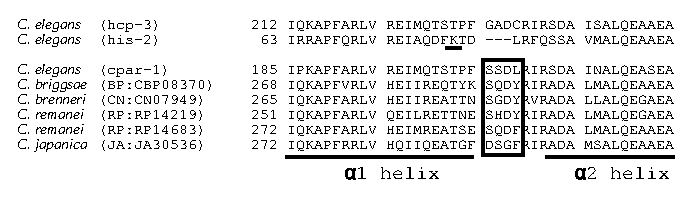
\includegraphics{Fig1}
\caption{Alignment of \protect\species{Caenorhabditis} \protect\mbox{CENP--A} homologues showing
conservation of possible PIKK recognition site inserted within H3 structure. The major
\protect\species{C\@. elegans} \protect\mbox{CENP--A} homologue (\protect\mbox{hcp--3}) and a canonical
H3 isoform (\protect\mbox{his--2}) with lysine 79 underlined are shown above.}
\label{fig:h2ax-review:celegans}
\end{figure}

\subsection{H2AX Gene}
Canonical histone genes in humans are spread over one large and two small clusters named HIST1,
HIST2 and HIST3. These are located at 6p21--p22, 1q21 and 1q42 respectively (\tref{tab:h2ax-review:H2A-localisation}).
Canonical H2A is encoded by sixteen genes, twelve of which are located in HIST1, three in HIST2 and
one in HIST3. H2A variants are located outside these histone clusters in the human genome, with the
H2AX--encoding gene H2AFX at 11q23.2--11q23.3 \citep{IZP+94} (\tref{tab:h2ax-review:H2A-localisation}).
Histone variant gene names typically include the letter F for family.

\begin{table}
\centering
\caption{Localisation of all human canonical and variant H2A genes and proteins (adapted from \protect\citet{WFM+02})}
\label{tab:h2ax-review:H2A-localisation}
\begin{tabular}{l l l l}
\toprule
Histone cluster & Gene & Protein & Locus  \\
\midrule
HIST1 & H2A A--E, G--M  & H2A.1           & 6p21--22\\
HIST2 & H2A A--C        & H2A.1 and H2A.2 & 1q21\\
HIST3 & H2A             & H2A.1           & 1q42\\
---   & H2AFB3          & H2ABbd          & Xq28\\
---   & H2AFJ           & macroH2A2       & 12p12\\
---   & H2AFV           & H2A.F/Z         & 7p13\\
---   & H2AFX           & H2AX            & 11q23.2--11q23.3\\
---   & H2AFY           & macroH2A1       & 5q31.3--q32\\
---   & H2AFZ           & H2A.Z           & 4q24\\
\bottomrule
\end{tabular}
\end{table}

The H2AFX promoter region, \SI{151}{\bp} upstream from the transcription start site, shows higher activity
than the typical canonical H2A.1 HIST1H2AE promoter in transcription reporter assays \citep{VSI94}.
There are two CCAAT elements upstream of the TATA box in H2AFX (\fref{fig:h2ax-review:H2AFX}) compared to a
single CCAAT element in the H2A.1. The CCAAT element proximal to the TATA box in H2AFX has a
significant effect on expression, whereas this element has no apparent effect on promoter activity
in the canonical H2A promoter. The transcription factors that bind to the element also bind to the
distal CCAAT as well as to three similar elements in H2AFZ but not to the one in the H2A.1 promoter \citep{VSI94}.
This suggests that H2AFX is regulated independently of canonical H2A.

\begin{figure}
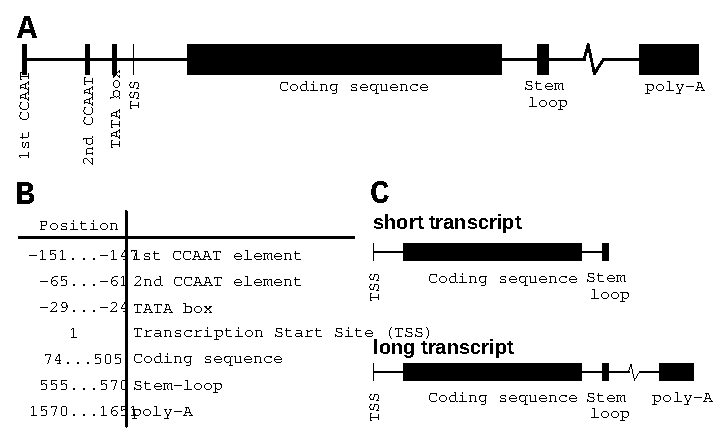
\includegraphics{Fig2}
\caption{H2AFX gene and transcripts. A.~Schematic of H2AFX gene region showing promoter and  3' mRNA
stabilizing elements. B.~Sequence coordinates of each element in H2AFX relative to transcription
start site\@. C.~Alternative transcripts of H2AFX\@. The short transcript  ($\approx$\SI{600}{\bp} in size) ends
in a stem--loop like canonical histones, whereas the long transcript ($\approx$\SI{1600}{\bp} in size) ends
in a poly--(A) tail.}
\label{fig:h2ax-review:H2AFX}
\end{figure}

\subsection{H2AX Transcripts}
A fundamental distinction between histone types is whether their expression is replication-dependent
or replication-independent. This difference is a consequence of the requirement for large amounts of
canonical histones during S~phase to package the newly duplicated genome (i.~e.\ replication-dependence).
In contrast, variant or ``replacement'' histones often appear to be inserted into chromatin to replace
canonical histones for functional reasons throughout the cell cycle and are therefore replication-independent \citep{WFM+02}.

Canonical histone genes lack introns, probably to circumvent the requirement for primary transcript
processing when histones must be rapidly produced at S~phase. A number of transcript features appear
to enhance the capacity of replication-dependent histone expression by up to 35-fold during S~phase.
In fact, there is only a five-fold increase in their transcription rate at S phase, compared to the
other phases of cell cycle so regulation acts strongly at the post-transcriptional level \citep{MEH+91}.
Replication-dependent histone transcripts lack a poly(A) tail and encode a stem--loop followed by a
purine-rich Histone Downstream Element (HDE) downstream of the stop codon. The stem--loop interacts
with the Stem--Loop Binding Protein (SLBP) to stabilise the mRNA in S~phase \citep{MLW+00} while the
HDE interacts with U7~snRNA to direct  efficient 3' end processing \citep{GB85}.

Human H2AX transcripts exhibit characteristics of both replication-dependent and replication-independent
histones. The H2AFX gene lacks introns, and has two alternative transcripts: one shorter form contains
the characteristic stem--loop, and the other longer form contains a downstream poly(A) tail \citep{CMWMB89}
(\fref{fig:h2ax-review:H2AFX}). The combined synthesis of H2AX transcripts has been described as ``weakly
replication-linked at best'' since the H2AFX promoter keeps the levels of both transcripts high
through the cell cycle \citep{VSI94}. However, the cell cycle linkage of the forms is unclear and no
study has reported the effect of DNA damage on transcription levels.

\subsection{H2AX Protein}
\label{subsec:h2ax-review:H2AX-protein}
Despite the large amount of attention paid to the DNA damage-linked serine phosphorylation by PIKKs,
the H2AX protein itself has a number of additional unique properties.

The defining feature of H2AX is considered to be the C--terminal region with the SQ[E/D]\textPhi motif
(\fref{fig:h2ax-review:H2AX-logo}). As mentioned in \Sref{subsec:h2ax-review:relation-H2A-H2AX}, the number of
residues separating this motif from the histone fold is variable and claimed to correlate with the
evolutionary complexity of the organism \citep{CRDP+02}. The residues responsible for this variable
spacing are mainly hydrophilic with a high glycine and proline content suggesting a flexible,
unstructured nature so the basis for the correlation could be more directly related to a structural
constraint such as the variation in internucleosomal repeat lengths of organisms which itself shows
linkage with evolutionary complexity.

\begin{figure}
%% FIXME  we want the side caption to appear on the outside. However, setting
%%        this to "outer" (default), seems to put it on the inside.  So we are
%%        reversing the logic by why is it failing?
\sidecapmargin{inner} % put memoir figure's sidecaption on the outerside
\setsidecappos{t}
\begin{sidecaption}{Sequence logo of all human canonical H2A isoforms showing differences with H2AX below. The
4 residues changes from H2A to H2AX outside the C--terminal region are Gln\,6\,Thr, Thr\,16\,Ser, Asn\,38\,His
and Lys\,99\,Gly. Alignment of H2A genes was made usign edialign \protect\citep{Mor99} from EMBOSS
\protect\citep{RLB00} and WebLogo 3 \protect\citep{CHC+04}.}[fig:h2ax-review:H2AX-logo]
\centering
\includegraphics[height=\textheight]{Fig3}
\end{sidecaption}
\end{figure}

In addition to the C--terminal motif, amino acid residues 6, 16, 38 and 99 of H2AX are different
from the human H2A.1 consensus (\fref{fig:h2ax-review:H2AX-logo} and \fref{fig:h2ax-review:H2AInNucleosome}). Inspection
of the human and \species{X.\ laevis} histone based nucleosome structures reveals that H2A residue~6 is
located in the flexible N--terminal tail and residue~16 is located at the very base of the tail
(\fref{fig:h2ax-review:H2AInNucleosome} and \fref{fig:h2ax-review:framed}b) which tracks the minor groove at superhelical
location~4.5 (SHL4.5) (\fref{fig:h2ax-review:framed}a). The substitution of glutamine with threonine at
position~6 in H2AX introduces a potential hydroxyl site for post-translational modification that is
not present for the glutamine in canonical H2A. In contrast, the threonine to serine substitution
conserves the modifiable hydroxyl at position~16.

\begin{figure}
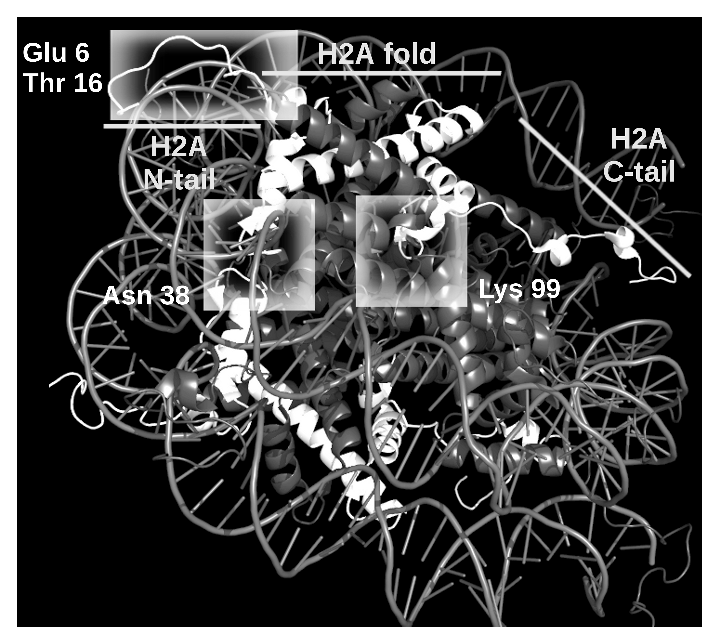
\includegraphics{Fig4}
\caption{Nucleosome structure highlighting differences between H2A and H2AX\@. H2A chain is
highlighted and white frames indicate the position of the residues that differ between the human
canonical H2A and H2AX\@. Image from PDB structure 1KX5 using PyMOL \protect\citep{DeL02}.}
\label{fig:h2ax-review:H2AInNucleosome}
\end{figure}

\begin{figure}
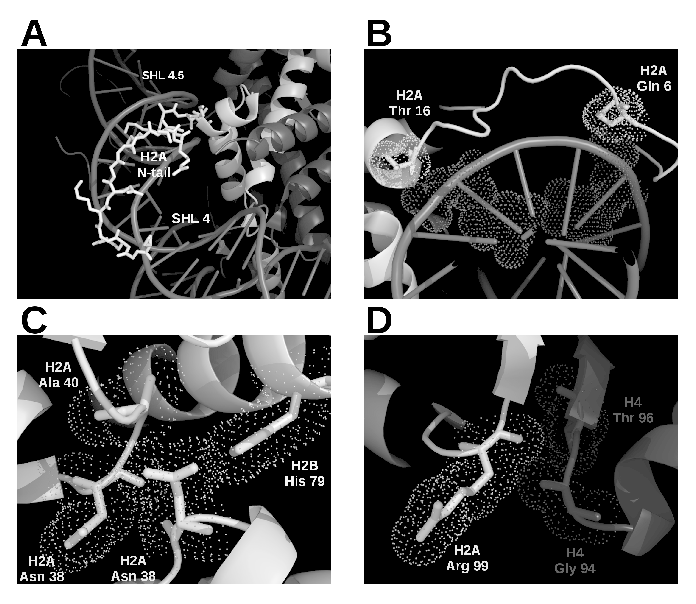
\includegraphics{Fig5}
\caption{Structural environment of H2A residues that differ from H2AX\@. The van der Waals surface
of differences and all residues within \SI{5}{\angstrom} are shown as a surface of dots over bond sticks. Image
from PDB structure 1KX5 using PyMOL \protect\citep{DeL02}. A.~H2A N--terminal tail encompassing H2AX
residues Thr\,6 and Ser\,16 passes across minor groove at superhelical location (SHL) 4.5\@. B.~Closeup
of H2A N--terminal tail minor groove association from A showing canonical H2A Gln\,6 and Thr\,16 which
become, respectively, Thr\,6 and Ser\,16 in H2AX\@. C.~Residues around H2A--H2A association in structure
showing interaction between paired Asn\,38 sidechains and adjacent residues. Canonical H2A Asn\,38 is
His\,38 in mammalian H2AX\@. D.~Environment around H2A Arg\,99 showing unusual absence of close packing.
Canonical H2A Arg\,99 is Gly\,99 in H2AX.}
\label{fig:h2ax-review:framed}
\end{figure}

Asparagine~38 is located in the loop between the \textalpha 1 and \textalpha 2 helices of H2A within the
nucleosome (\fref{fig:h2ax-review:H2AInNucleosome} and \fref{fig:h2ax-review:framed}c). Importantly, this residue makes
direct contact with the equivalent amino acid in the other H2A--H2B dimer in the nucleosome structure
and has been suggested to affect both nucleosome stability and the balance between homotypic and
heterotypic combinations (see \Sref{subsec:h2ax-review:H2AX-distribution}) of H2A types within the yeast
nucleosome \citep{CLW01}. It is possible that the change of residue~38 from asparagine in H2A to
histidine in H2AX could also affect nucleosome stability and dynamics. For example, weakening of
interactions between the two H2A-H2B histone fold dimers could result in increased nucleosome
flexing and impact the ability to condense into stable higher order chromatin structure. Furthermore,
the presence of the histidine in H2AX could affect the stabilisation of a second copy of H2AX
relative to canonical H2A within the nucleosome. This change of asparagine to histidine at
position~38 occurs only in higher organism H2AX and could potentially drive a bias towards either
homotypic H2AX-only or heterotypic H2AX--H2A mixed nucleosomes which could have consequences for the
distribution of H2AX in chromatin (see \Sref{subsec:h2ax-review:H2AX-distribution}).

The effect of the final substitution distinguishing canonical H2A and H2AX where lysine becomes
glycine at position~99 is less clear. This residue is located in a sharp turn immediately after
the \textalpha 3 helix and points towards the C--terminal ends of H3 and H4 but makes no direct
interactions in the nucleosome (\fref{fig:h2ax-review:H2AInNucleosome} and \fref{fig:h2ax-review:framed}d). Nevertheless,
the exchange of the large, positively charged and potentially modifiable lysine for the highly
flexible glycine in H2AX could potentially alter stability and flexibility of the nucleosome.

\subsection{H2AX Post-Translational Modifications}
\label{subsec:h2ax-review:H2AX-PTM}
Histones typically have a large proportion of amino acid residues which are modified post-translationally
for functional reasons so it is significant that three of the four residues distinguishing human H2A
and H2AX in the core region are capable of distinction via post-translational modification
(i.~e.\ Thr\,6 and Ser\,16 in H2AX vs.\ Thr\,16 and Lys\,99 in canonical H2A).

However, only the phosphorylation of H2AX serine 139 by PIKKs in response to DNA damage has been
intensively studied. This modification has been demonstrated to enhance access of restriction
enzymes and DNA methylases to the DNA, possibly by reducing nucleosome stability \citep{KHHK+08}. In
the same study the activity of the FACT complex which can facilitate dissociation of H2A/H2B dimers
from nucleosomes was shown to increase after H2AX phosphorylation.

One of the most recently reported post-translational modifications of H2AX related to DSB is the
phosphorylation of tyrosine~142 in the PIKK recognition motif of human H2AX \citep{XLS+09,CJT+09}. In
contrast to the phosphorylation of Ser\,139, this Tyr\,142 residue is phosphorylated under normal
conditions with DNA damage acting as trigger for its dephosphorylation. The dephosphorylation seems
to not only precede the phosphorylation of Ser\,139, but also to be a prerequisite for the Ser\,139
phosphorylation. When Tyr\,142 is phosphorylated, affinity of Ser\,139 to the DNA damage response
factors MDC1, MRE11 and Rad50 is greatly reduced and binding by pro-apoptopic factor JNK1 was found
to occur instead. It has therefore been suggested that the phosphorylation status of Tyr\,142 is a
determinant of cell fate after DNA damage.

H2AX can also be subject of acetylation at lysine~5 \citep{PB81} and to both mono- and poly-ubiquitylation
at lysine~119 dependent on the prior acetylation at Lys\,5 (\tref{tab:h2ax-review:H2AX-PTM}) \citep{ITK+07}. These
modifications are intimately related to DNA repair because their levels increase significantly after
exposure to DSB-inducing Ionising Radiation (IR) and appear to drive H2AX eviction from the nucleosome
by the action of Tip60 complex and UBC13 \citep{ITK+07}. However, conflicting data about the
interdependence of these effects with phosphorylation has recently been reported \citep{RVD+09}.

\begin{table}
\centering
\caption{Reported Post-Translational Modifications (PTMs) for H2AX\@. Other PTMs present in H2A but
not yet related to H2AX include acetylation of lysine 9 and 13 \protect\citep{ZEP+03}, phosphorylation
of threonine 120 \protect\citep{ANY+04}, and the possible methylation of lysine 127 \protect\citep{ZEP+03}.}
\label{tab:h2ax-review:H2AX-PTM}
\begin{tabular}{r l l l l}
\toprule
Residue number & Residue indentity & PTM & Related to DSB  & Reference  \\
\midrule
1   & Serine & phosphorylation & no  & \citet{PB81} \\
5   & Lysine    & acetylation     & yes & \citet{PB81} and \citet{ITK+07} \\
9   & Lysine    & biotinylation   & no  & \citet{CCK+06} \\
13  & Lysine   & biotinylation   & no  & \citet{CCK+06} \\
119 & Lysine  & ubiquitylation  & yes & \citet{ITK+07} \\
139 & Serine  & phosphorylation & yes & \citet{EPR+98} \\
142 & Tyrosine  & phosphorylation & yes & \citet{XLS+09} \\
\bottomrule
\end{tabular}
\end{table}

Other modifications unrelated to DNA damage have been reported for H2AX, including a rather unusual
biotinylation of Lys\,9 and Lys\,13 \citep{CCK+06} and the phosphorylation of Ser\,1 \citep{PB81}. By
homology to canonical H2A, it is probable that Lys\,9 and Lys\,13 can also be acetylated \citep{ZEP+03}
and Thr\,120 phosphorylated \citep{ANY+04}. Another interesting possible post-translational modification
is a methylation at Lys\,127 \citep{ZEP+03}. Although it was inconclusive whether Lys\,125 or Lys\,127
is the target of this methylation, it is tempting to speculate that it occurs at Lys\,127 since this
residue is the only one conserved in the C--terminal of all human H2A sequences (\fref{fig:h2ax-review:H2AX-logo}).

\subsection{H2AX Distribution in Chromatin}
\label{subsec:h2ax-review:H2AX-distribution}
The original estimates of H2AX abundance in human cells reported cell line specific values from
\SIrange{2.5}{25}{\percent} of total H2A in asynchronous immortalised cell lines \citep{EPR+98}. These values were
determined by densitometry of Coomassie-stained, acid-extracted histones in two-dimensional gels. A
\pcent{10} abundance value of H2AX has become accepted despite wide differences in the study and the fact
that HeLa cells were reported to contain \pcent{2.5} H2AX\@.

Although it is tempting to interpret \pcent{10} abundance as implying every tenth nucleosome will contain
H2AX, combinatorial features of nucleosomes make the statistics of spacings between H2AX occurrences
in the chromatin fibre more complex. H2AX can be incorporated either as one or as two copies per
nucleosome (\fref{fig:h2ax-review:H2AX-distribution}A), and the H2AX-containing nucleosomes can be either
randomly or non-randomly distributed along the chromatin fibre (\fref{fig:h2ax-review:H2AX-distribution}B--C).
Random incorporation would lead not simply to each tenth nucleosome containing H2AX, but to a
geometric distribution of spacings between H2AX-containing nucleosomes. This predicts many instances
of small spacings and some instances of very large spacings, and has clear implications for the
ability of \textgamma H2AX to signal local damage events as well as for the spreading of the
phosphorylation along the chromatin fibre.

\begin{figure}
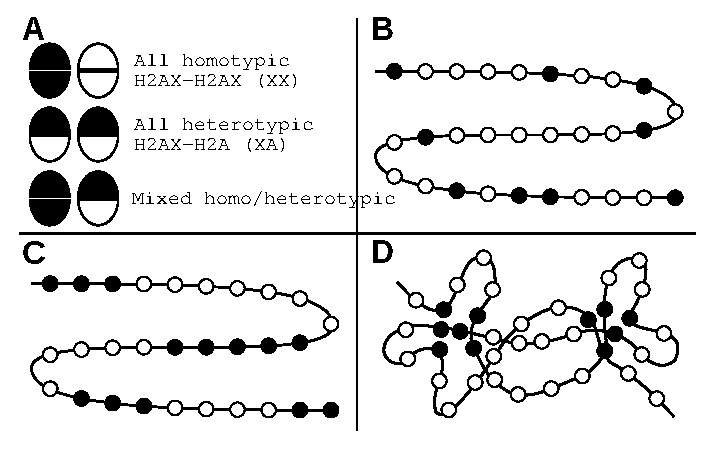
\includegraphics{Fig6}
\caption{H2AX distribution in the chromatin. A.~Schematic of possible H2AX homotypic, heterotypic and
mixed nucleosome combinations. Black semicircle represents H2AX--H2B dimer and white semicircle
represents H2A--H2B dimer. B.~Random incorporation of H2AX into nucleosomes would lead to a random
distribution of H2AX-containing nucleosomes. C.~Selective incorporation of H2AX into nucleosomes
would lead to ``islands'' of H2AX-containing nucleosomes. D.~Random incorporation of H2AX nucleosomes
could also lead to ``islands'' of H2AX nucleosomes by chromatin reorganization.}
\label{fig:h2ax-review:H2AX-distribution}
\end{figure}

\subsubsection{Combinatorial potential in H2AX distribution}
The combinatorial potential for H2AX inclusion has two separate features which could affect the
detailed distribution of H2AX along chromatin.

Firstly, either one or two H2AX polypeptides can in principle be present within a nucleosome: Two
H2AX copies would give rise to a ``homotypic'' H2AX/H2AX (`XX') nucleosome, whereas a single H2AX
copy will give rise to a ``heterotypic'' H2AX/H2A (`XA') nucleosome (\fref{fig:h2ax-review:H2AX-distribution}A).
It is currently unknown whether there is a bias for either homotypic or heterotypic nucleosomes
(see \Sref{subsec:h2ax-review:H2AX-protein}) although this affects the statistics of H2AX spacing in
chromatin since the XA combination yields twice as many H2AX-containing nucleosomes than XX for a
given H2AX abundance.

Secondly, the spacing of nucleosomes containing H2AX should have a major influence on its functional
roles in DSB signaling, assembling of repair foci and facilitating the repair machinery. H2AX
nucleosomes could be randomly distributed (\fref{fig:h2ax-review:H2AX-distribution}B) or subject to clustering
in one (\fref{fig:h2ax-review:H2AX-distribution}C) or three dimensions (\fref{fig:h2ax-review:H2AX-distribution}D). Any
mechanism randomly assembling chromatin from pools of XX and/or XA versus canonical H2A--H2A (`AA')
nucleosomes will give rise to a geometric distribution of spacings between H2AX (\fref{fig:h2ax-review:H2AX-graphs}A).
This distribution predicts a bias towards small spacings (\fref{fig:h2ax-review:H2AX-graphs}A).

\begin{figure}
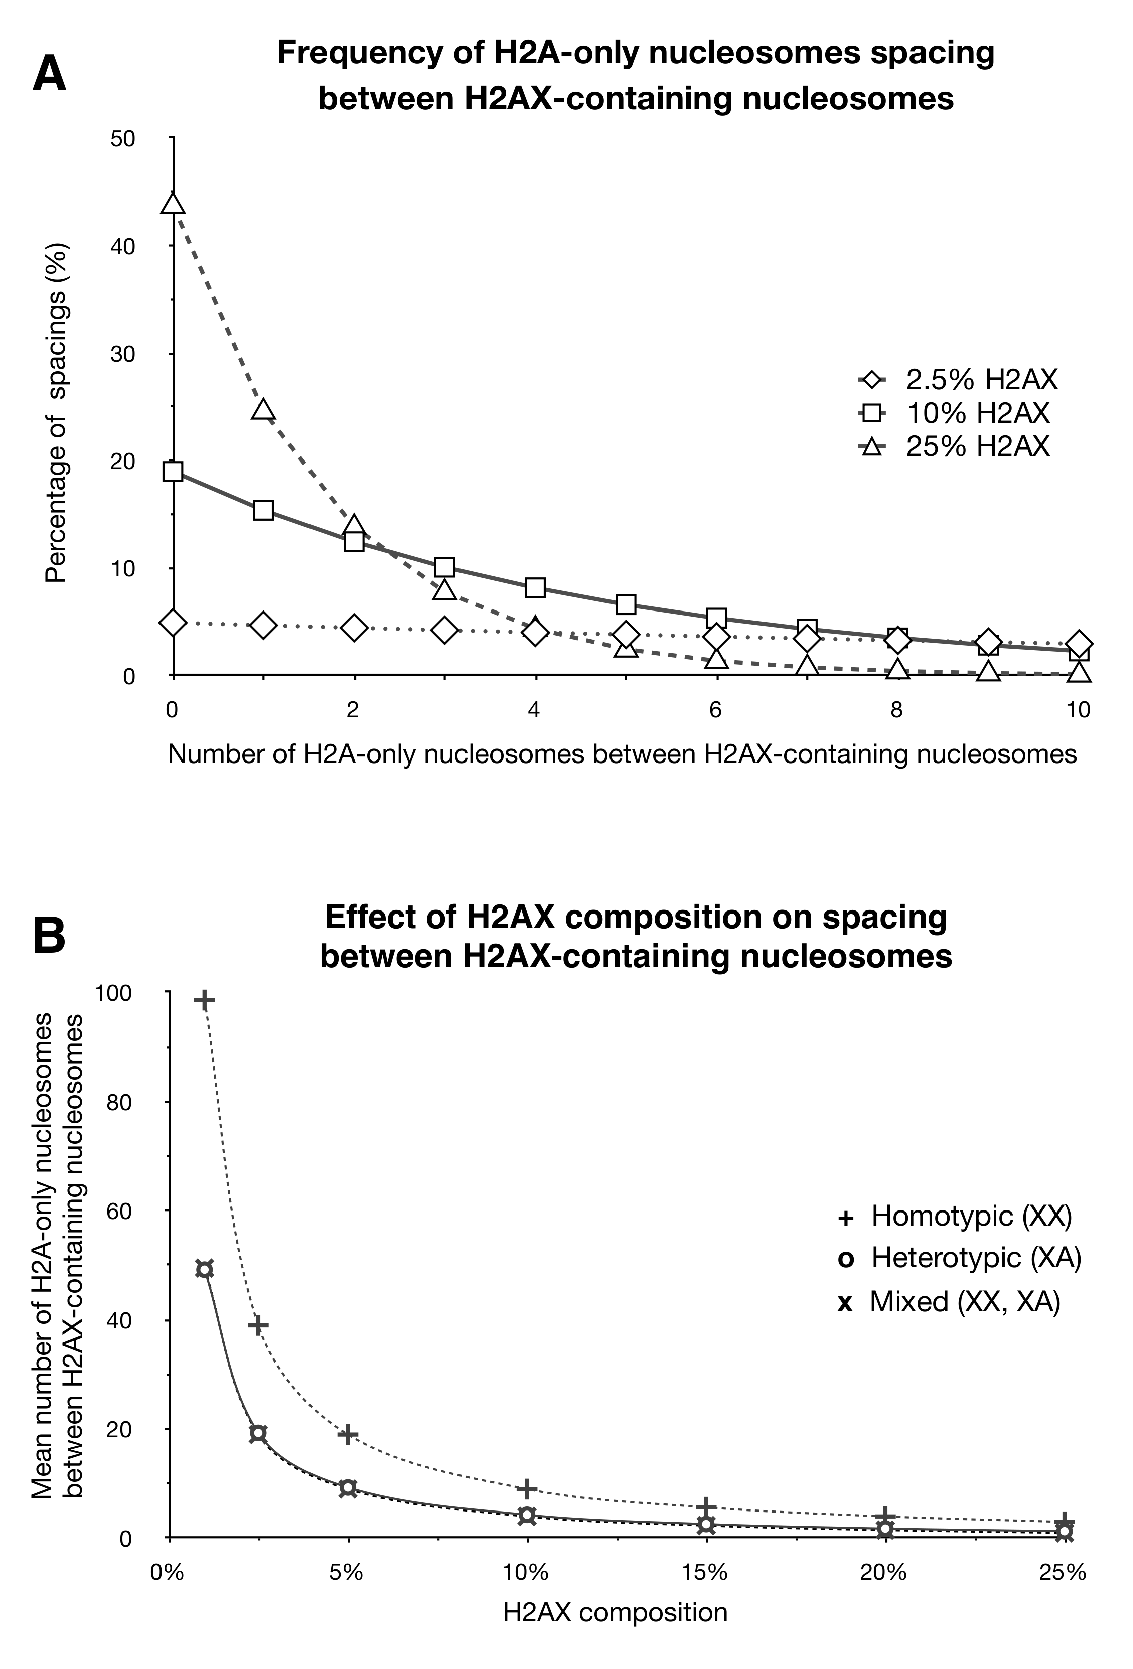
\includegraphics[width=\textwidth]{Fig7}
\caption{Simulations of H2AX spacing distributions. A.~Distribution of spacings between instances of
H2AX for mixed population of homotypic and heterotypic nucleosomes at abundances of \pcent{2.5} (dot),
\pcent{10} (solid) and \pcent{25} (dashed) H2AX in total H2A pool. B.~Effect of abundance on mean H2AX spacing
for homotypic (H2AX--H2AX) only, heterotypic (H2AX--H2A) only, and mixed homotypic$+$heterotypic
nucleosome combinations.}
\label{fig:h2ax-review:H2AX-graphs}
\end{figure}

\subsubsection{Simulation of random H2AX inclusion}
Simple computational simulations reveal interesting features in this H2AX spacing distribution. In
the simplest case of H2AX assembling in a mixture of XA and XX nucleosomes, \pcent{10} overall H2AX
abundance would generate an average of 4.3 nucleosomes between H2AX occurrences along the chromatin
fibre (\fref{fig:h2ax-review:H2AX-graphs}B). The mean spacing is highly sensitive to H2AX abundance
(\fref{fig:h2ax-review:H2AX-graphs}A), so \pcent{2.5} and \pcent{25} H2AX abundances yields means of 19.3 to 1.3
nucleosomes, respectively (\fref{fig:h2ax-review:H2AX-graphs}B). Similar results arise for calculations
where only heterotypic XA nucleosomes can assemble and homotypic XX nucleosomes are structurally
precluded. In contrast, if heterotypic XA nucleosomes are precluded and only XX nucleosome
structures can assemble, then \pcent{10} H2AX abundance yields a mean spacing of 9 nucleosomes between
H2AX occurrences. The mean spacings for \pcent{2.5} and \pcent{25} H2AX abundance are 39 to 3 nucleosomes
respectively (\fref{fig:h2ax-review:H2AX-graphs}B).

\subsubsection{Functional implications of H2AX distribution}
These simple models of random nucleosome incorporation have interesting implications. The occurrence
of occasional large H2AX spacings could limit both processive \textgamma H2AX spreading along the
chromatin fibre and the proximity of H2AX in solenoidal higher order chromatin packaging. At \pcent{10} H2AX
abundance, \pcent{23} of nucleosomes in mixed XA and XX nucleosomes will be spaced by more than 6 nucleosomes
and in the extreme case of \pcent{2.5} H2AX abundance, \pcent{84} of solely homotypic XX nucleosomes would be
spaced by more than 6 nucleosomes.

This sensitivity of H2AX spacing in chromatin to abundance provides a potential opportunity for the
cell to regulate responsiveness to damage. For example, if H2AX expression is up-regulated the mean
proximity of randomly inserted H2AX will rapidly increase and effects such as processive \textgamma H2AX
spreading and retention of DDR factors at foci will be significantly enhanced.

It is unknown whether H2AX distribution varies between euchromatin and heterochromatin. However,
differences in H2AX response have been reported according to the condensation level of chromatin and
phosphorylation of Ser\,139 has been observed to occur preferentially in euchromatin \citep{IGC+07}.
This preference is overcome during replication of heterochromatin when it is in a less condensed
state \citep{IGC+07}. The distinction between active and inactive chromatin can also be regulated, as
demonstrated for phosphorylation of KAP--1 by ATM reducing the access of DNA repair proteins to
heterochromatic regions of the genome \citep{AAG+08}.

\subsubsection{Possibility of non-random H2AX distribution}
If H2AX nucleosome incorporation is not a random process (\fref{fig:h2ax-review:H2AX-distribution}B),
inhomogeneity could also exist at a more local level. For example, small ``islands'' of higher
density H2AX nucleosomes could be interspersed within broader regions with lower relative abundance
of the variant (\fref{fig:h2ax-review:H2AX-distribution}C). A recent study using a novel high-resolution
microscopy observed several thousand small spatial clusterings of H2AX and pointed to a mutual
exclusivity of H2AX and the phosphorylated form \citep{JBBTB06}. This would be consistent with a
clustering model (\fref{fig:h2ax-review:H2AX-distribution}D) that enhanced the kinetics of the damage
signaling at foci, perhaps by making use of a chromatin structural feature such as the chromosomal
scaffold \citep{JBBTB06}. The inherent clustering and active insertion of H2AX in the DDR could also
drive larger scale chromosomal rearrangements through chromatin stability (\fref{fig:h2ax-review:H2AX-distribution}D) \citep{KHHK+08}.

\section{Functional Roles of H2AX}
Phosphorylation of H2AX serine 139 by PIKKs to generate ``\textgamma H2AX foci'' is an early and
characteristic feature of DSB events. This modification is thought to be the primary identifier of
the location of DNA damage and would therefore be central to the function of H2AX.

The \textgamma H2AX foci extend for \SIrange{2}{30}{\mega\bp} along the chromatin fibre \citep{EPR+99}, implying the
involvement of a span of \numrange{e4}{e5} nucleosomes per individual DSB repair event. At \pcent{10} H2AX
abundance, this would involve up to \numrange{e2}{e4} H2AX molecules and hence a \numrange{e2}{e4} fold
amplification of DSB event signal. A direct link between the site of a lesion and a single focus has
been observed \citep{KRIK+03}, suggesting that there is a linkage between \textgamma H2AX and the repair
mechanism. Many protein factors have been identified, which depend directly or indirectly on the
phosphorylation of H2AX at serine 139. Thereafter, it appears to act as a foundation for recruitment
of DDR factors at DSB sites \citep{TTP+00}. As a consequence, H2AX performs a role in both localisation
and structuring of the repair focus.

\subsection{Initiation of H2AX Phosphorylation as a Reporter of DSB Events}
The process of establishing H2AX phosphorylation at the characteristic terminal motif can be performed
by any of the three PIKKs ATM, ATR and DNA--PK\@. Their induction and binding characteristics suggest
that H2AX phosphorylation for focus generation can be distinguished by an initiation phase when a
small number of phosphorylations are made at nucleosomes adjacent to the break, and a spreading phase
in which a larger region of phosphorylation extends one-dimensionally from either side of the break.
The structural exposure of the serine 139 site through chromatin flexibility will be crucial determinant
of the modification event (see \Sref{subsec:h2ax-review:H2AX-PTM}).

ATM has been considered a strong candidate as the principal kinase responsible for the initiation phase
of general damage events because it responds to changes in chromatin conformation expected when a
spontaneous DSB event releases local superhelical tension \citep{CJB03}. ATR appears to be linked to
replication stress or UV damage events which lead to breaks as indirect consequences, so ATR is recruited
by ATRIP which detects single-stranded DNA\@. DNA--PK is localised to DSBs in complex with the end-binding
protein Ku, so such an association will act to limit the distance from the damaged end on which DNA--PK
can act \citep{WCG01} and such an end-dependent mechanism would be sensitive to H2AX abundance and distribution.

\subsection{Spreading of H2AX Phosphorylation as a Damage Signal Amplifier}
The conventional model for \textgamma H2AX focus formation suggests that after initiation in the
immediate vicinity of the break by ATM and/or DNA--PK, amplification occurs by spreading through the
action of MDC1 binding to \textgamma H2AX \citep{MSJAC+05}. MDC1 in turn recruits the MRN complex
(Mre11--Rad50--Nbs1) via direct interaction with Nbs1 \citep{LMS+04} and the MRN complex further activates
ATM \citep{ULM+03}. This generates a positive feedback loop to drive spreading of the phosphorylation
modification away from the break. Hence H2AX acts both as signal and target of phosphorylation in the
spreading phase. Each focus acts independently even when several foci are formed in the immediate
vicinity of each other \citep{MJK+06}, suggesting a one dimensional diffusion along the chromatin fibre.

How the signal spreads over megabase but non-infinite distances is unknown. It is possible that
non-homogeneous H2AX distribution could contribute to the localisation of \textgamma H2AX stochastically
through random occurrence of large spacings between H2AX that the spreading mechanism could not bridge
(see \Sref{subsec:h2ax-review:H2AX-distribution}). Consistent with this, high resolution microscopy reveals
that H2AX is not randomly distributed but organized into discrete clusters which would control the
expansion of the signal \citep{JBBTB06}.

Since levels of phosphorylated H2AX rise rapidly in response to damage and then reduce over time \citep{EPR+98}
it is necessary to remove either the phosphate or the entire \textgamma H2AX\@. The timing of this process
is unclear but must depend on the presence of \textgamma H2AX binding factors such as MDC1 which could
stabilise \textgamma H2AX or obscure the phosphate group \citep{MSJAC+05}. In \species{S.\ cerevisiae},
dephosphorylation is achieved by removal of phosphorylated H2AX from nucleosomes and subsequent
dephosphorylation by the HTP--C complex \citep{MKJK+06}. In higher eukaryotes the mechanisms remain
unclear since several phosphatases have been implicated in the process and these can variously
dephosphorylate H2AX within nucleosomes or after removal \citep{CKI+05,KTA+06,CXZ+08}. In addition,
the FACT complex which facilitates nucleosome exchange has enhanced activity on phosphorylated H2AX \citep{KHHK+08}
suggesting at least one pathway involving displacement for extra-nucleosomal dephosphorylation. A
background level of H2AX remains phosphorylated even in the apparent absence of DNA damage, but the
reason for this is unknown \citep{EPR+98}.

\subsection{\textgamma H2AX and Chromatin Structural Remodelling}
Intrinsically, H2AX phosphorylation must take place within the context of chromatin structure so
both the Non-Homologous End Joining (NHEJ) and Homologous Recombination (HR) pathways can efficiently
undertake DSB repair. To facilitate this, chromatin decondenses near the DSB \citep{MJK+06} but the
mechanism for this remodeling is unclear.

The modified serine 139 of H2AX is located near the DNA entry/exit point on the nucleosome
(\fref{fig:h2ax-review:H2AInNucleosome}) so one putative mechanism for the chromatin structural change is to
be driven directly by the chemical properties of the added phosphate group. \species{S.\ cerevisiae}
mutants with the serine 139 equivalent mutated to glutamate to mimic the phosphate charge show
increased micrococcal nuclease sensitivity consistent with such a destabilisation \citep{JAD00} and
phosphorylated human H2AX renders chromatin more susceptible to restriction enzymes and DNA
methylase \citep{KHHK+08}. However, a separate analysis of chromatin structure, also in yeast,
harboring the glutamate mutation did not find evidence of direct chromatin structural effects \citep{FIT07}.

An alternative indirect mechanism for linking H2AX phosphorylation with chromatin disruption is by
recruitment of proteins to drive remodeling. A number of different ATP-dependent chromatin remodeling
activities have been implicated in this process, including RSC, SWI/SNF, INO80 and SWR (reviewed
in \citet{JAD07}), as well as other nucleosome modifying enzymes such as the NuA4 histone
acetyltransferase. There is also evidence that chromatin chaperones and binding proteins contribute
to the process of chromatin dynamics at DSBs. For example, the FACT complex, which participates in
exchange between H2A and H2AX, has greater ability to mobilise \textgamma H2AX than unphosphorylated
H2AX \citep{KHHK+08}. In addition, HP1\textbeta, which binds to H3~K9me, has recently been shown to be
released by phosphorylation immediately after DSB events and that this contributes to H2AX
phosphorylation by PIKKs \citep{AJB+08}.

Both direct and indirect mechanisms for chromatin remodeling depend on H2AX phosphorylation, and
hence require an independent initiation step. The PIKKs ATM and DNA--PK can achieve this by
detecting changes in chromatin structure or appearance of DNA ends, respectively \citep{CJB03,BC04}.
However, the impact of chromatin on PIKK initiation is difficult to probe because H2AX phosphorylation
occurs very rapidly after DSBs, making it difficult to temporally distinguish factors which remodel
chromatin to enable initial PIKK access from downstream events which undertake remodeling to
amplify \textgamma H2AX around the site.

Furthermore, despite the intimate link between H2AX phosphorylation and chromatin remodeling at the
DSB site, local decondensation of chromatin occurs at similar levels on both wild type and H2AX$^{-/-}$ cell
lines when ATP is not depleted \citep{MJK+06}. This suggests that the role of H2AX phosphorylation in
driving the chromatin remodeling is redundant with other pathways.

\subsection{\textgamma H2AX and Localisation of DSB Repair Proteins}
Since H2AX phosphorylation is one of the earliest events after a DSB, this suggests it may play a
role in subsequent recruitment of the active repair proteins. This is supported by the absence of
RAD51 and BRCA1 at DSB foci when \textgamma H2AX phosphorylation is prevented \citep{TTP+00}. However,
NBS1, BRCA1 and 53BP1 are recruited to the sites of damage in H2AX$^{-/-}$ cell lines which display
only moderate sensitivity to ionising radiation but fail to maintain focal localisation \citep{ACOF+03}.
It has therefore been suggested that the crucial role of H2AX phosphorylation is not as a direct agent
of repair factor recruitment, but of retention of these factors in the vicinity of the DSB \citep{ACOF+03}.
This role in defining a ``damage neighborhood'' does not necessarily imply a direct role in repair at
the break site itself. For example, stimulation of the G2/M checkpoint may result from the accumulation
of checkpoint signalling factors at the focus \citep{OFHC+02}. In fact, Chromatin ImmunoPrecipitation
(ChIP) revealed that \textgamma H2AX is evicted from the region close to the DSB early in the DDR in
\species{S.\ cerevisiae} and that \textgamma H2AX does not strictly co-localise with the active repair
complexes \citep{RSAA+04}.

This accumulated retention of DDR factors in the vicinity of a DSB appears to be a complex process
where the initiating damage signal is integrated by factors recognising the H2AX phosphorylation and
presumably additional chromatin features. For example, human 53BP1 and its putative homologues,
\species{S.\ cerevisiae} Rad9 and \species{S. pombe} Crb2, all contain Tudor domains which bind specific
methylated histones in chromatin, and BRCT domains which can both mediate dimerisation and bind
\textgamma H2AX\@. Despite the similarity in domain structure of Rad9, Crb2 and 53BP1, individual
investigations have indicated that they have different binding capabilities. The Rad9 Tudor domain
binds H3~K79me \citep{GCJ+07,HZDJ+04} whereas Crb2 and 53BP1 Tudor domains bind H4~K20me2 \citep{SPM+04,BLW+06}.
Rad9 and Crb2 BRCT domains bind directly to \textgamma H2AX \citep{HMH+07,KDR+08} whereas 53BP1 does not,
instead relying on an indirect interaction mediated by the BRCT domain of MDC1 which directly binds
\textgamma H2AX \citep{MSL+05,MSJAC+05}. Some direct interaction between 53BP1 BRCT domain and \textgamma H2AX
has also been reported by co-precipitation studies, but in a much smaller proportion than Rad9 and
Crb2 \citep{KDR+08}. Rad9 and Crb2 can all also dimerise or oligomerise through their BRCT domains \citep{SL99,DMR04}
although this domain is not necessary for the oligomerisation of 53BP1 \citep{AWX+05}. The latter
instead requires a sequence upstream of its Tudor domain \citep{WKM+06}.

This complex interplay between the combinatorial interactions made by 53BP1, Rad9 and Crb2 with
themselves and with \textgamma H2AX builds up to generate another level of the structural environment
for the repair process. \textgamma H2AX therefore acts as a foundation to define the extent of the
repair focus through the H2AX distribution and the extent of its phosphorylation.

\subsection{\textgamma H2AX and Maintenance of Proximity of Break Ends}
Linked to this role in retaining repair factors in the repair focus, phosphorylated H2AX also appears
to function in the bringing together of damaged ends. It has been suggested that by recruiting repair
factors which directly associate with the damaged ends, H2AX could prevent diffusion of these ends
away from each other \citep{BA04}. For example, linkage has been observed in the distribution of
cohesin and \textgamma H2AX near DSBs \citep{UAS+04} so \textgamma H2AX-dependent cohesin association would
promote the stabilisation of sister chromatids to facilitate HR\@. Furthermore, localisation of
self-interacting factors by their association with \textgamma H2AX nucleosomes could bring together
distant break ends. For example, 53BP1 is suggested to localise to break ends by direct interaction
with nucleosomes and indirect interaction through MDC1 \citep{HZDJ+04,BLW+06,EAR+09}. Oligomerisation
of 53BP1 has also been reported to enhance association of distant ends, thereby facilitating long
range recombination and NHEJ \citep{DGW+08,DCS+08}.

\subsection{\textgamma H2AX and Complementary Damage Signalling Via Ubiquitylation}
A secondary pathway of signaling by ubiquitylation of both canonical H2A and H2AX has recently been
uncovered which appears to derive directly from \textgamma H2AX, and therefore act as a complementary
amplification of the damage signal \citep{PD09}. Recognition of H2AX phosphorylation by MDC1 leads to
recruitment of an initiating ubiquitylation by RNF8 and UBC13 which is subsequently amplified with
the involvement of RNF158, and possibly maintained by Rap80 and BRCT1\@. The direct role of the
ubiquitylation remains to be clarified because it can act in factor recruitment as well as affecting
the structure, stability or turnover of histones including H2AX itself.

\section{Conclusion}
Despite H2AX having a highly similar primary sequence or even overlapping identity with canonical H2A,
it is clear that the DNA damage-linked function of this histone variant is highly specific. Its
functional role is as an amplifier of the damage event signal, a foundation for marshaling repair
factors, and a promoter of the chromatin dynamics required to complete the repair process. It is
clear that the phosphorylation of serine 139 by PIKKs generates an epitope which is crucial to these
functions. Nevertheless, it is important to note that the DNA damage response is only moderately
defective in H2AX$^{-/-}$ cells, suggesting that complementary mechanisms must operate redundantly
with H2AX functions. Much remains to be appreciated about \textgamma H2AX structure and function, but
this must ultimately be based on the unique distinguishing features of the H2AX gene and protein.

\subsubsection*{Acknowledgements}
We thank Prof.\ Cathal Seoighe for assistance with calculations of random H2AX distribution,
Prof.\ Noel Lowndes for his input and Dr.\ Kevin Roche for helpful discussions. We gratefully
acknowledge the support of Science Foundation Ireland and Health Research Board of Ireland for
supporting work in our laboratory. DMSP acknowledges the support of the Portuguese Foundation for
Science and Technology (FCT).




  \backmatter

  \bibliography{%
    intro/references,%
    methods/references,%
    histone-catalogue/references,%
    kill-frap/references,%
    fancy-frap/references,%
    h2ax-review/H2AXreview-biblio%
  }

\end{document}
